%!TEX TS-program = pdflatex
%!TEX encoding = UTF-8 Unicode

% Reference.tex, part of the Pipmak Game Engine
% Copyright (c) 2004-2011 Christian Walther
% 
% This program is free software; you can redistribute it and/or modify
% it under the terms of the GNU General Public License as published by
% the Free Software Foundation; either version 2 of the License, or
% (at your option) any later version.
% 
% This program is distributed in the hope that it will be useful,
% but WITHOUT ANY WARRANTY; without even the implied warranty of
% MERCHANTABILITY or FITNESS FOR A PARTICULAR PURPOSE.  See the
% GNU General Public License for more details.
% 
% You should have received a copy of the GNU General Public License
% along with this program; if not, write to the Free Software
% Foundation, Inc., 51 Franklin St, Fifth Floor, Boston, MA  02110-1301  USA

% $Id: Reference.tex 231 2011-10-30 07:23:30Z cwalther $

%\input protcode.tex

\documentclass[
	a4paper,
	pagesize,
	10pt,
	oneside,
	%openany, openright
	%draft,
	idxtotoc,
	bibtotoc,
	BCOR10mm,
	DIV10
]{scrartcl} %scrreprt
\pagestyle{plain} %plain/empty/headings
\setkomafont{sectioning}{\normalfont\normalcolor\bfseries}
\deffootnote{1em}{1em}{\thefootnotemark\ }
\setkomafont{caption}{\sffamily\small}
\setkomafont{captionlabel}{\bfseries}
%\addtokomafont{caption}{\small}

\usepackage[english]{babel}
\usepackage[utf8]{inputenc}
\usepackage[T1]{fontenc}
%\usepackage{units}
\usepackage{makeidx}
\makeindex
%\usepackage{showidx}
\usepackage{fancyvrb}
\usepackage{graphicx}
\usepackage{color}
\definecolor{linkblue}{rgb}{0,.2,.6}
\usepackage[
	pdftex,
	a4paper,
	breaklinks,
	hyperindex,
	colorlinks,
	linkcolor=linkblue,
	filecolor=linkblue,
	pagecolor=linkblue,
	urlcolor=linkblue,
	bookmarks=true,
	bookmarksopen=true,
	bookmarksnumbered=true,
	pdfhighlight=/O,
	pdfsubject={Pipmak version 0.2.7},
	pdftitle={Pipmak Reference},
	pdfauthor=CWalther,
	pdfstartview=FitH
]{hyperref}
\usepackage{ae}
\usepackage{amsfonts} %for mathbb
\usepackage{textcomp} %seems to be required for \textdegree after updating my TeX installation
\usepackage[noBBpl]{mathpazo}
\renewcommand{\ttdefault}{pcr}
\renewcommand{\sfdefault}{cmbr}

%\subject{...}
\title{Pipmak 0.2.7 Reference}
\author{Christian Walther \textsf{‹\href{mailto:cwalther@gmx.ch}{cwalther@gmx.ch}›}}
%\date{...} %default is \today

\def\dotfill{\leaders\hbox to.6em{\hss .\hss}\hskip 0pt plus 1fill} %from doc.sty

% \luafunction{TABLE}{FUNCTION}{ARGUMENTS}
% Example: \luafunction{pipmak}{gotonode}{nodename [, inbackground]}
% \luafunction is for making a heading for a Pipmak Lua function's
% documentation.  It formats the function name and its parameters as a
% heading in a box.
\newcommand{\luafunction}[3]{\noindent\hypertarget{#1.#2}{\setlength{\fboxsep}{1ex}\fbox{\texttt{#1.#2(\textit{#3})}\index{#2@\texttt{#2}}\index{#1 functions@\texttt{#1} functions!#2@\texttt{#2}}}}\\}

% \luamethod{TYPE}{METHOD}{ARGUMENTS}
% Exmample: \luamethod{node}{setstandardcursor}{cursor}
% \luamethod is for making a heading for the documentation for a
% method of a Pipmak Lua object (also called "userdata type").
\newcommand{\luamethod}[3]{\noindent\hypertarget{#1:#2}{\setlength{\fboxsep}{1ex}\fbox{\texttt{\textit{#1}:#2(\textit{#3})}\index{#2@\texttt{#2}}\index{#1 methods!#2@\texttt{#2}}}}\\}

% \luadescription{DESCRIPTION}
% All Pipmak Lua function descriptions should be pased to
% \luadescription, after using \luafunction to create a heading for
% the function, in order for then to be formatted properly.
\newcommand{\luadescription}[1]{\sloppy\begin{addmargin}[0.1\textwidth]{0pt}#1\end{addmargin}\vspace{2ex}\fussy}

% \luaconstant{TABLE}{CONSTANT}
% Example: \luaconstant{pipmak}{left}
% Whenever a Pipmak Lua constant is referred to, \luaconstant should
% be used to format it properly.
\newcommand{\luaconstant}[2]{\texttt{#1.#2}\index{#2@\texttt{#2}}\index{#1 constants@\texttt{#1} constants!#2@\texttt{#2}}}
\newcommand{\luaconstantshort}[2]{\texttt{#2}\index{#2@\texttt{#2}}\index{#1 constants@\texttt{#1} constants!#2@\texttt{#2}}}

\newcommand{\ttindex}[1]{\index{#1@\texttt{#1}}}
\newcommand{\ttindexed}[1]{\texttt{#1}\index{#1@\texttt{#1}}}
\newcommand{\emphindexed}[1]{\emph{#1}\index{#1}}

% \luaparam{PARAMATER}
% Example: \luaparam{image} is the file name...
% Parameter names, in bodies of text, should be formatted with
% \luaparam.
\newcommand{\luaparam}[1]{\texttt{\textit{#1}}}

% \lualink{FUNCTION}
% Example: \lualink{pipmak.gotonode}.
% \lualink creates a link to the description of a specified Pipmak Lua
% function.  Should be used whenever a function is referred to in a
% body of text.
\newcommand{\lualink}[1]{\hyperlink{#1}{\texttt{#1}}}

% \luamethodlink{METHOD}
% Example: \luamethodlink{node}{setstandardcursor}
% \luamethodlink is the same as \lualink, but for userdata methods.
\newcommand{\luamethodlink}[2]{\hyperlink{#1:#2}{\texttt{#2}}}

\renewcommand{\url}[1]{\textsf{‹\href{#1}{#1}›}}

\newcommand{\secref}[1]{\ref{sec:#1} “\nameref{sec:#1}”}

\newcommand{\todo}[1]{\marginline{\emph{{\footnotesize TO DO:} {\small #1}}}}


\begin{document}
%\setprotcode\font
%{\it \setprotcode\font}
%{\bf \setprotcode\font}
%{\bf \it \setprotcode\font}
%\pdfprotrudechars=1

\maketitle
\vspace{2cm}
\begin{center}
\includegraphics[width=10cm]{figures/pipmak.png}\end{center}
\newpage
\tableofcontents
\newpage

\section{Introduction}
Pipmak is an open-source cross-platform game engine and authoring environment for point-and-click adventure games in the style of the \emph{Myst} series, including panoramic ones like \emph{Myst III: Exile}. Pipmak binaries for various platforms as well as Pipmak's source code can be downloaded from \url{http://pipmak.sourceforge.net/}. There you'll also find information on how to reach Pipmak's developers and fellow Pipmak users through the mailing lists/newsgroups.

Making a game using Pipmak is mostly a matter of creating the game's graphics using a 3D rendering program or other graphics software and then describing to Pipmak how these should be presented and how they should behave in specially formatted text files. At the current state of development, there is not much editing that can directly be done in Pipmak, so calling it an “authoring environment” may be a bit of a stretch. This is planned to change in future versions, though. You can, however, edit a project while it is running in Pipmak and immediately see your changes.

This document is the reference documentation for Pipmak. It is currently unfinished and incomplete. Once finished, it will contain detailed descriptions and specifications of everything you need to know about Pipmak's features. It does not contain documentation about the non-Pipmak-specific parts of the scripting language Lua that is used by Pipmak because such documentation is available elsewhere (see section \secref{scripting}). Neither is it a tutorial that will walk you through creating a game using Pipmak. Such a tutorial does not exist at the moment (although you're welcome to write one). Instead, a demo project that shows all of Pipmak's features in action is available.

If you find that some information in this manual is incorrect, please report it so that it can be corrected, or submit a fix yourself. The \LaTeX{} source code for this document is available in Pipmak's source code distribution and in the Subversion repository. Also, please report if you find some parts to be incomprehensible. This document is being written by Pipmak's developer, who occasionally may neglect properly explaining what seems obvious to him, and is thankful for such cases being pointed out to him.

\section{Pipmak Projects}
\label{sec:projects}

\subsection{General Structure and Terminology}
Projects consist of a set of \emph{nodes}\index{node}, which can either be panoramic or flat. Flat nodes include \emph{slides}\index{slide} that fill the whole screen, and rectangular \emph{panels}\index{panel} that can be displayed on top of other nodes. The background image/panorama of each node is constant, but \emph{patches}\index{patch} can be placed on it to modify the image in response to user actions, game state, or dynamically. The node contains areas named \emph{controls}\index{control} that react to mouse actions (click, drag, enter, leave etc.) by invoking scripts that may be as simple as going to another node or as complex as required for a complete puzzle. There are two types of controls: \emph{hotspots}\index{hotspot}, which are static, can have any shape, and are defined by an image file, and \emph{handles}\index{handle}, which are rectangular, movable, and are defined in Lua code only. In the simplest case, exactly one node is shown at any time (the \emphindexed{background node}), but it is also possible to display other nodes (\emph{overlays}\index{overlay}) on top of the background node to achieve such effects as head-up displays, picture frames, or floating inventory windows.

\subsection{Filesystem Organization}
Pipmak projects are not stored in opaque files, but in a folder structure that is meant to be human-readable. In fact, setting up this structure manually is currently the only way of creating a project.

A Pipmak project is stored in a folder whose name ends with “.pipmak”. Such a folder is automatically made into a package (a folder that's presented like a file by the Finder) on Mac OS X—to get at its contents, ctrl-click on it and choose “Show Package Contents” from the contextual menu. On other operating systems, the project appears as an ordinary folder.

Inside the project folder, each node is stored as a folder containing its resources (image files etc.) and a Lua file \emphindexed{node.lua} describing its properties and containing its scripts. These folders may be placed in arbitrarily nested subfolders to structure the project and can bear arbitrary names with the exception of the following: reserved for internal use are the top-level folders \emph{0}, any starting with \emph{-}, \emph{resources}, \emph{modules}, \emph{pipmak}, \emph{pipmak\_internal}, as well as all subfolders of those. Additionally, the project contains a Lua file \emphindexed{main.lua} that controls global properties of the project. The Lua files are plain text files that can be created and modified using any text editor. Basic text editors, such as TextEdit on Mac OS X or Notepad on Windows, are usually included with every OS.

An example of a project with three nodes (“node1”, “A”, “B”) and additional data files is shown in figure \ref{fig:filesystem}.

\begin{figure}[htbp]
\centering
\setlength{\fboxsep}{3mm}
\fbox{
{\small
\begin{tabular}{l@{\hspace{2cm}}l}
\textbf{Filesystem layout} & \textbf{Relative path as seen from node A}\\[4bp]
\hline
\raisebox{-3bp}{
\includegraphics{figures/icon-project.png}} \textsf{Project.pipmak} & \rule{0pt}{3.5ex}\\[2bp]
\qquad \raisebox{-3bp}{
\includegraphics{figures/icon-folder.png}} \textsf{\textbf{node1}} & \texttt{\textit{"../node1"}} \\[2bp]
\qquad \qquad \raisebox{-3bp}{
\includegraphics{figures/icon-png.png}} \textsf{background.png} & \texttt{"../../node1/background.png"} \\[2bp]
\qquad \qquad \raisebox{-3bp}{
\includegraphics{figures/icon-lua.png}} \textsf{node.lua} &\\[2bp]
\qquad \raisebox{-3bp}{
\includegraphics{figures/icon-folder.png}} \textsf{more} &\\[2bp]
\qquad \qquad \raisebox{-3bp}{
\includegraphics{figures/icon-folder.png}} \textsf{\textbf{A}} & \texttt{\textit{"A"}} \\[2bp]
\qquad \qquad \qquad \raisebox{-3bp}{
\includegraphics{figures/icon-jpeg.png}} \textsf{node.jpeg} & \texttt{"node.jpeg"} \\[2bp]
\qquad \qquad \qquad \raisebox{-3bp}{
\includegraphics{figures/icon-lua.png}} \textsf{node.lua} &\\[2bp]
\qquad \qquad \qquad \raisebox{-3bp}{
\includegraphics{figures/icon-folder.png}} \textsf{patches} &\\[2bp]
\qquad \qquad \qquad \qquad \raisebox{-3bp}{
\includegraphics{figures/icon-png.png}} \textsf{patch35.png} & \texttt{"patches/patch35.png"} \\[2bp]
\qquad \qquad \raisebox{-3bp}{
\includegraphics{figures/icon-folder.png}} \textsf{\textbf{B}} & \texttt{\textit{"B"}} \\[2bp]
\qquad \qquad \qquad \raisebox{-3bp}{
\includegraphics{figures/icon-jpeg.png}} \textsf{b.jpeg} & \texttt{"../B/b.jpeg"} \\[2bp]
\qquad \qquad \qquad \raisebox{-3bp}{
\includegraphics{figures/icon-lua.png}} \textsf{node.lua} &\\[2bp]
\qquad \raisebox{-3bp}{
\includegraphics{figures/icon-lua.png}} \textsf{blah.lua} & \texttt{"../../blah.lua"} \\[2bp]
\qquad \raisebox{-3bp}{
\includegraphics{figures/icon-folder.png}} \textsf{foo} &\\[2bp]
\qquad \qquad \raisebox{-3bp}{
\includegraphics{figures/icon-jpeg.png}} \textsf{bar.jpeg} & \texttt{"../../foo/bar.jpeg"} \\[2bp]
\qquad \raisebox{-3bp}{
\includegraphics{figures/icon-lua.png}} \textsf{main.lua} &\\[2bp]
\end{tabular}
}}
\caption{Filesystem organization example}\label{fig:filesystem}
\end{figure}

For distribution, projects can be archived into a single ZIP file, whose name should end with “.pipmak” as well (not “.zip”, since that might lead users to believe that they must unzip it). The layout of a zipped project is exactly the same as for a non-zipped project folder, just that “Project.pipmak” (in the example of figure \ref{fig:filesystem}) now is a ZIP archive instead of a folder. In other words, when zipping up a project, you must put the \emph{contents} of the project folder (node folders, \emph{main.lua}, etc.) into the archive, not the project folder itself.

\subsubsection{Specifying Paths}
\label{sec:specifyingpaths}
At several places in the \emph{node.lua} file describing a node you are expected to specify the names (actually, paths) of certain data files such as panorama faces and hotspot maps. You can place such files anywhere inside the project. Typically files used in only one node are placed in that node's folder, and those used in several nodes are placed at the top level of the project or subfolders thereof. There are two ways of referring to a file:

\textbf{Absolute path:} Specify the full path from the top level of the project to the file, starting with \texttt{/} and using \texttt{/} as the folder separator (example: \texttt{"/more/A/patches/patch35.png"} in figure \ref{fig:filesystem}).

\textbf{Relative path:} Anything not starting with \texttt{/} is interpreted in relation to the node in whose \emph{node.lua} you are:
\begin{itemize}
\item For a file that is located in the node's folder, you just provide the file name (example: \texttt{"node.jpeg"} in figure \ref{fig:filesystem}).
\item If the file is located in a subfolder of the node folder, specify the path to it, using \texttt{/} as the folder separator (example: \texttt{"patches/patch35.png"} in figure \ref{fig:filesystem}).
\item If the file is located outside of the node, e.g.\ at the top level of the project or in another node, use “\texttt{../}” in the path to get up to the containing folder as many times as needed (examples: \texttt{"../../node1/background.png"}, \texttt{"../B/b.jpeg"} etc.\ in figure \ref{fig:filesystem}). “\texttt{..}” cannot be used to get to files outside of the project, extraneous occurrences are ignored.
\item As an exception, when referring to other nodes rather than data files (e.g.\ in the \lualink{pipmak.gotonode} function), relative paths are interpreted as relative to the parent folder of the current node folder, not the current node folder itself (examples: \texttt{\textit{"../node1"}}, \texttt{\textit{"A"}}, \texttt{\textit{"B"}} in figure \ref{fig:filesystem}). This allows sibling nodes to refer to each other simply by name.
\end{itemize}

Make sure to use the correct capitalization in paths. Referring to a file called \emph{Sound.ogg} as \texttt{"sound.ogg"} will work on the default file systems of Mac OS X and Windows if your project is a folder, but not on Linux or if the project is zipped.

Paths specified in \emph{main.lua} are always relative to the top level of the project, i.e.\ you need not start them with “\texttt{/}” to get to the top (but you can).

Most often your paths will be literal strings, i.e.\ characters surrounded by quotation marks as in the examples above, but don't forget that \emph{node.lua} is an ordinary Lua file and you can use any Lua expression that evaluates to a string where a path is expected. Obviously, this also applies to numbers and all other parameters.

\subsubsection{Supported File Formats}
\textbf{Image files:} Pipmak can read all image files supported by the SDL\_image library. Currently, these are: BMP, PNM (PPM/PGM/PBM), XPM, LBM, PCX, GIF, JPEG, PNG, TGA, TIFF.

\textbf{Sound files:} Currently, Pipmak only understands a single sound file format: Ogg Vorbis. See \url{http://www.vorbis.com/software/} for a list of applications that can help you with creating Ogg Vorbis sounds or reencoding your existing sounds in Vorbis.

\subsection{How Pipmak Finds Projects}
When Pipmak is started without the user specifying a project to open (e.g. by doubleclicking a project in the file manager or naming it on the command line), it looks for files or folders with names ending in \emph{.pipmak} in the following places, in that order:
\begin{itemize}
\item Pipmak's own resources folder/archive. On Mac OS X, that's the folder \emph{Pipmak.app\,/ Contents\,/\,Resources\,/}, on Windows and Linux it's the ZIP archive \emph{Pipmak Resources} next to the application.
\item The folder that contains the Pipmak application.
\item All mounted CDs.
\end{itemize}

Pipmak then tries to open the first such file or folder found. If none is found, or if the first one found is not a proper Pipmak project, it displays the usual main menu instead.

So, to make a standalone project, you'd put your project into the resources folder or archive, or if you want one package that includes applications for all platforms, place it next to the applications. 

\subsection{Project Properties}
Global properties of a project are specified in the Lua file \emphindexed{main.lua} that sits at the top level of the project.

A project needs a title, which is displayed in the window title bar and which is used to identify to what project a saved game belongs. Additionally, Pipmak needs to know which node to show when the project is opened. These properties are specified by the following statements in \emphindexed{main.lua}, where \luaparam{title} and \luaparam{nodename} are strings, \luaparam{nodename} a path as explained in section \secref{specifyingpaths}:
\hypertarget{title}{}\ttindex{title}\hypertarget{startnode}{}\ttindex{startnode}
\begin{Verbatim}[frame=single, framesep=1ex, xleftmargin=0.1\textwidth, xrightmargin=0.1\textwidth, commandchars=\\^\$]
title \textit^title$
startnode \textit^nodename$
\end{Verbatim}
Currently, the title may only contain ASCII characters. Any accented letters or other special characters will be replaced by question marks. 

Optionally, you can specify which version of Pipmak you used when designing the project, by writing
\hypertarget{version}{}\ttindex{version}
\begin{Verbatim}[frame=single, framesep=1ex, xleftmargin=0.1\textwidth, xrightmargin=0.1\textwidth, commandchars=\\^\$]
version (\textit^version$)
\end{Verbatim}
in \emphindexed{main.lua}. \luaparam{version} is a decimal number with the major version number as integer part and the minor and sub-minor version numbers as the first and second decimal place. The user then gets a warning if his version of Pipmak is older or significantly newer than the version specified in the project. The general rule is that a new version of Pipmak will get a new minor version number if it introduces incompatibilities with projects made for the last version, while only the sub-minor revision number is incremented if older projects continue to work.

Lua code that should be executed every time the project is opened can be placed in an \ttindexed{openproject} handler in \emphindexed{main.lua}:
\hypertarget{onopenproject}{}\ttindex{onopenproject}
\begin{Verbatim}[frame=single, framesep=1ex, xleftmargin=0.1\textwidth, xrightmargin=0.1\textwidth, commandchars=\\^\$]
onopenproject (
  function()
    \textit^--do something$
  end
)
\end{Verbatim}
This is the place to initialize the game state stored in the \ttindexed{state} table (see section \secref{storinggamestate}).

While it will currently work placing such code directly in \emphindexed{main.lua}, this is deprecated because \emphindexed{main.lua} may also be run on other occasions in a future version.

\subsection{Node Properties}
Lua code that should be executed every time a certain node is entered can be placed in a function set as an \ttindexed{enternode} handler in the corresponding \emphindexed{node.lua}:
\hypertarget{onenternode}{}\ttindex{onenternode}
\begin{Verbatim}[frame=single, framesep=1ex, xleftmargin=0.1\textwidth, xrightmargin=0.1\textwidth, commandchars=\\^\$]
onenternode (\textit^function$)
\end{Verbatim}
Uses of \texttt{enternode} handlers include initializing local state variables, starting timers (see section \secref{timing}) to do background animation, or displaying overlays (see section \secref{nodemethods}). You can define multiple \texttt{enternode} handlers, they will be called in the order of their definition when the node is entered.

While it will currently work placing such code directly in \emphindexed{node.lua}, this is deprecated because \emphindexed{node.lua} may also be run on other occasions in a future version.

To run some Lua code on leaving a node, use \ttindexed{leavenode} handlers:
\hypertarget{onleavenode}{}\ttindex{onleavenode}
\begin{Verbatim}[frame=single, framesep=1ex, xleftmargin=0.1\textwidth, xrightmargin=0.1\textwidth, commandchars=\\^\$]
onleavenode (\textit^function$)
\end{Verbatim}

The \texttt{enternode} handlers are also called when nodes are entered during the process of loading a saved game. If this is a problem because some of the initializations done in the \texttt{enternode} handler are already in effect in the state loaded from the saved game file and should not be redone, set a flag in the \lualink{state} table at the end of the \texttt{enternode} handler and clear it in the \texttt{leavenode} handler. Then check that flag at the beginning of the \texttt{enternode} handler and skip the initialization if it is already set, indicating that we are coming from a saved game rather than another node.

When several nodes are displayed simultaneously (see section \secref{thenodestack}), \ttindexed{mouseenter} and \ttindexed{mouseleave} handlers allow you to track on which one the mouse pointer currently is:
\hypertarget{onmouseenter}{}\ttindex{onmouseenter}\hypertarget{onmouseleave}{}\ttindex{onmouseleave}
\begin{Verbatim}[frame=single, framesep=1ex, xleftmargin=0.1\textwidth, xrightmargin=0.1\textwidth, commandchars=\\^\$]
onmouseenter (\textit^function$(\textit^node$))
onmouseleave (\textit^function$(\textit^node$))
\end{Verbatim}

The mouse is considered to be inside an overlay\index{overlay} node when either the background of that node is opaque or less than half transparent at the mouse location, or when it has a control under the mouse location. (So, to make a node that's more than half transparent catch mouseenter and mouseleave events, cover it with a dummy hotspot or handle.)

\subsection{Slides}
\label{sec:slides}

A slide node consists of a single rectangular background image that is scaled to fill the Pipmak window (or the screen in fullscreen mode), optionally adding black bars at the sides if necessary to preserve the aspect ratio. To make a slide node, write either of
\hypertarget{slide}{}\ttindex{slide}\ttindex{border}\ttindex{cursor}\hypertarget{mousemode}{}\ttindex{mousemode}
\begin{Verbatim}[frame=single, framesep=1ex, xleftmargin=0.1\textwidth, xrightmargin=0.1\textwidth, commandchars=\\^\$]
slide \textit^image$
\end{Verbatim}
\begin{Verbatim}[frame=single, framesep=1ex, xleftmargin=0.1\textwidth, xrightmargin=0.1\textwidth, commandchars=\\^\$]
slide {
  \textit^image$,
  [border = \textit^boolean$,]
  [cursor = \textit^cursor$,]
  [mousemode = \textit^mode$]
}
\end{Verbatim}
as the first statement of \emph{node.lua}.

\luaparam{image} is the file name (or path) of an image file (see section \secref{specifyingpaths}). Alternatively, \luaparam{image} may also be an image object obtained from the \lualink{pipmak.getimage} or \lualink{pipmak.newimage} functions (it then needs to be put in parentheses in the first form because Lua only allows the parentheses to be omitted around string literals).

The \luaparam{border} property controls what happens when the slide's aspect ratio doesn't match the screen's (or window's) aspect ratio. If it is \texttt{true}, black bars are added to the sides of the slide. This is the default. If it is \texttt{false}, the border is transparent. This is mainly useful when the slide is displayed as an overlay on top of another node (see section \secref{thenodestack}).

The optional \luaparam{cursor} property specifies a mouse cursor to be used on this node instead of the global standard cursor (see section \secref{mousecursors}). It must either be one of the predefined constants listed in table~\ref{tab:cursors} on page \pageref{tab:cursors}, or a cursor object obtained from the \lualink{pipmak.loadcursor} function.

Providing a \luaparam{mousemode} (which must be either \luaconstant{pipmak}{joystick} or \luaconstant{pipmak}{direct}, see \lualink{pipmak.setmousemode}) is a shortcut for adding the code below to \emph{node.lua}: the mouse mode will be set to the given value as long as this node is displayed, unless it is overridden again by another call to \lualink{pipmak.pushmousemode} or another node's \luaparam{mousemode} setting.
\begin{Verbatim}[frame=single, framesep=1ex, xleftmargin=0.1\textwidth, xrightmargin=0.1\textwidth, commandchars=\\^\$]
local token
onenternode (
  function() token = \lualink^pipmak.pushmousemode$(\textit^mode$) end
)
onleavenode (
  function() \lualink^pipmak.popmousemode$(token) end
)
\end{Verbatim}

\subsection{Panels}
\label{sec:panels}

A panel is a flat, rectangular node similar to a slide. The difference is that it is not scaled to fill the screen, but remains at screen resolution. Since panels usually only cover a part of the screen, they are most useful as overlays rather than background nodes (see section \secref{thenodestack}). Uses for panels include inventories, pop-up menus, and floating utility windows.

The background of a panel is given by an image file. The panel may be bigger or smaller than the image, but unlike slides, the image is not uniformly scaled in that case. Rather, the corners of the image stay fixed to the corners of the panel, and the space between them is filled with what's in the middle of the image. Imagine horizontally stretching the image with a left and a right margin of a certain width rigid and only the central part stretchable, then in the same way vertically stretching the result with rigid top and bottom margins. By default, these rigid margins each make up a whole half of the image, and only the center row or column of pixels is stretchable. (If the image's width or height are an even number of pixels, which of the two middle rows or columns is used is undefined. Either use odd dimensions, or make sure that the two middle rows/columns are identical.)

To make a panel node, use either of
\hypertarget{panel}{}\ttindex{panel}\ttindex{w}\ttindex{h}\ttindex{relx}\ttindex{rely}\ttindex{absx}\ttindex{absy}\ttindex{cursor}
\begin{Verbatim}[frame=single, framesep=1ex, xleftmargin=0.1\textwidth, xrightmargin=0.1\textwidth, commandchars=\\^\$]
panel \textit^image$
\end{Verbatim}
\begin{Verbatim}[frame=single, framesep=1ex, xleftmargin=0.1\textwidth, xrightmargin=0.1\textwidth, commandchars=\\^\$]
panel {
  \textit^image$,
  [w = \textit^width$,]
  [h = \textit^height$,]
  [leftmargin = \textit^leftmargin$,]
  [rightmargin = \textit^rightmargin$,]
  [topmargin = \textit^topmargin$,]
  [bottommargin = \textit^bottommargin$,]
  [relx = \textit^relativex$,] [absx = \textit^absolutex$,]
  [rely = \textit^relativey$,] [absy = \textit^absolutey$,]
  [cursor = \textit^cursor$,]
  [mousemode = \textit^mode$]
}
\end{Verbatim}
as the first statement of \emph{node.lua}.

\luaparam{image} is the file name (or path) of an image file (see section \secref{specifyingpaths}). Alternatively, \luaparam{image} may also be an image object obtained from the \lualink{pipmak.getimage} or \lualink{pipmak.newimage} functions (in parentheses because Lua only allows the parentheses to be omitted around string literals).

\luaparam{w} and \luaparam{h} specify the size of the panel in screen pixels. If omitted, the image's width and height are used.

\luaparam{leftmargin}, \luaparam{rightmargin}, \luaparam{topmargin}, and \luaparam{bottommargin} specify the width or height in pixels of the margins that stay rigid when the panel is stretched to a different size than the image size. Default values are half the image width for left and right, and half the image height for top and bottom, so that only a vertical and a horizontal line in the center of the image stay stretchable, as discussed above.

The position of a panel on the screen consists of a relative part (in screen widths/heights) and an absolute part (in screen pixels). The left edge of the panel lies at \luaparam{relx} $\cdot\ screen\_width$ $+$ \luaparam{absx} pixels from the left edge of the screen, and its top edge at \luaparam{rely} $\cdot\ screen\_height\ +$ \luaparam{absy} pixels from the top edge of the screen. For example, \texttt{panel \{ w = 60, h = 40, relx = 1.0, absx = -60, rely = 0.0, absy = 15 \}} produces a panel whose right edge lies at the right edge of the screen and whose top edge is 15 pixels from the top of the screen. \texttt{panel \{ w = 90, h = 50, relx = 0.5, absx = -45, rely = 1.0, absy = -60 \}} centers the panel horizontally and positions its bottom edge 10 pixels from the bottom of the screen.

All of the positional properties are optional, default values are chosen as follows:
\begin{itemize}
\item If neither a relative nor an absolute position is specified, the panel is horizontally centered and vertically positioned at the top third of the screen.
\item If only a relative position is given, it is interpreted as “relative to the range within which the panel can move while still staying completely on screen”. That is, 0 aligns the left (top) edge of the panel at the left (top) edge of the screen, 0.5 centers the panel, and 1 aligns the right (bottom) edge of the panel at the right (bottom) edge of the screen. Therefore, the \texttt{absx} property could have been omitted in both of the above examples, without changing the result.
\item If only an absolute component is given, the relative component is set to 0, i.e. the specified number directly sets the left or top margin between panel and screen edge in pixels.
\end{itemize}

The optional \luaparam{cursor} property specifies a mouse cursor to be used on this panel instead of the global standard cursor (see section \secref{mousecursors}). It must either be one of the predefined constants listed in table~\ref{tab:cursors} on page \pageref{tab:cursors}, or a cursor object obtained from the \lualink{pipmak.loadcursor} function.

The \luaparam{mousemode} property specifies a mouse mode to be used while this node is displayed (see \lualink{pipmak.setmousemode}). It must be either \luaconstant{pipmak}{joystick} or \luaconstant{pipmak}{direct}. See the description of the same property in section \secref{slides} for details.


\subsection{Cubic Panoramas}
\label{sec:cubicpanoramas}

The six square faces of a cube onto which the scene has been projected along rays passing through the cube's midpoint form a cubic panorama. To make a cubic panorama node in Pipmak, write the following as the first statement of \emph{node.lua}, where \luaparam{face1} \ldots \luaparam{face6} are the file names (or paths, see section \secref{specifyingpaths}) of the six face images:
\hypertarget{cubic}{}\ttindex{cubic}\ttindex{cursor}
\begin{Verbatim}[frame=single, framesep=1ex, xleftmargin=0.1\textwidth, xrightmargin=0.1\textwidth, commandchars=\\^\$]
cubic {
  \textit^face1$, \textit^face2$, \textit^face3$, \textit^face4$, \textit^face5$, \textit^face6$,
  [cursor = \textit^cursor$,]
  [mousemode = \textit^mode$]
}
\end{Verbatim}

A face image can be mirrored by setting any of the options \luaparam{fliphorizontally} and \luaparam{flipvertically} to \texttt{true} on it. This is done by replacing the respective \luaparam{face} in the above syntax by a table containing it as the first element, along with the options:
\ttindex{fliphorizontally}\ttindex{flipvertically}
\begin{Verbatim}[frame=single, framesep=1ex, xleftmargin=0.1\textwidth, xrightmargin=0.1\textwidth, commandchars=\\^\$]
{ \textit^face$, [fliphorizontally = true,]
        [flipvertically = true] }
\end{Verbatim}


The optional \luaparam{cursor} property specifies a mouse cursor to be used on this node instead of the global standard cursor (see section \secref{mousecursors}). It must either be one of the predefined constants listed in table~\ref{tab:cursors} on page \pageref{tab:cursors}, or a cursor object obtained from the \lualink{pipmak.loadcursor} function.

The \luaparam{mousemode} property specifies a mouse mode to be used while this node is displayed (see \lualink{pipmak.setmousemode}). It must be either \luaconstant{pipmak}{joystick} or \luaconstant{pipmak}{direct}. See the description of the same property in section \secref{slides} for details.

The faces are numbered in the order \emph{front}, \emph{right}, \emph{back}, \emph{left}, \emph{top}, \emph{bottom}, with the top and bottom rotated 90\textdegree\ from the front view, as shown in figure~\ref{fig:facenumbers}. (This is the same ordering and orientation as is used in QuickTime VR.)

\begin{figure}[htbp]
\centering
\setlength{\fboxsep}{3mm}
\fbox{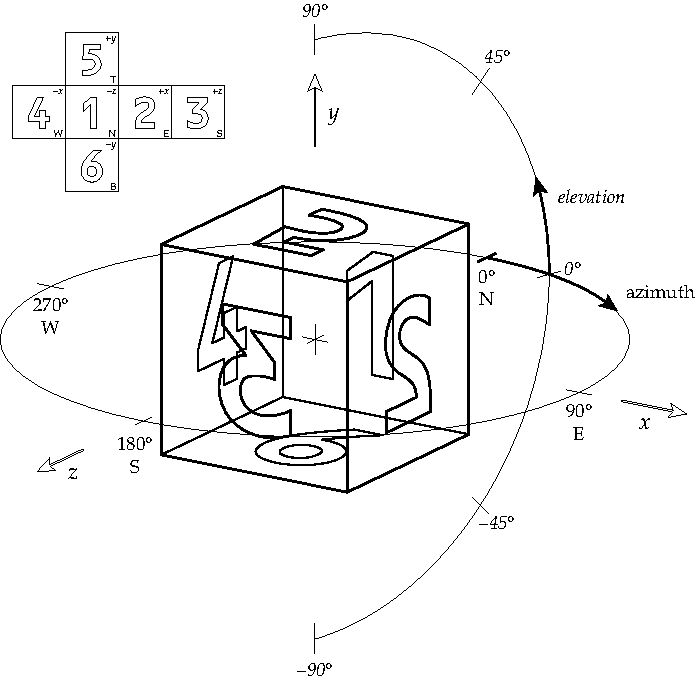
\includegraphics[width=0.5\textwidth]{figures/facenumbers.pdf}}
\caption{Ordering and orientation of the cube faces}\label{fig:facenumbers}
\end{figure}

Width and height of the images (in pixels) need not be the same (non-square images will be squished into square shape, making their pixels non-square), and different faces may have different sizes (you might use a lower resolution for the top and bottom than for the sides, for example). Reasonable sizes are between 512 $\times$ 512 and 1024 $\times$ 1024.

You may constrain the directions in which the viewer can look in a panorama by specifying minimum and maximum values for azimuth and elevation by placing the following statement in \emph{node.lua}:
\hypertarget{limits}{}\ttindex{limits}\ttindex{minaz}\ttindex{maxaz}\ttindex{minel}\ttindex{maxel}
\begin{Verbatim}[frame=single, framesep=1ex, xleftmargin=0.1\textwidth, xrightmargin=0.1\textwidth, commandchars=\\^\$]
limits {
  [minaz = \textit^number$,]
  [maxaz = \textit^number$,]
  [minel = \textit^number$,]
  [maxel = \textit^number$] 
}
\end{Verbatim}
The elevation limits should satisfy $-90 \leq \luaparam{minel} \leq \luaparam{maxel} \leq 90$. The azimuthal limits may both lie anywhere in the range [0, 360], the view is restricted to what lies to the right of \luaparam{minaz} and to the left of \luaparam{maxaz}. Default values are $-80, 80$ for elevation and 0, 360 (which amounts to an unlimited view) for azimuth. Each (panoramic) node has its own limits, there are no universal limits.

\minisec{Making Cubic Panoramas}
\label{sec:makingcubicpanoramas}
Since the cube faces are flat, projecting the scene onto them is an ordinary perspective projection, which is easily achieved in any 3D rendering program. Viewed from the middle of the cube, each face appears under a horizontal and vertical field of view of 90\textdegree. However, there is a small gotcha that will cause your panoramas to look wrong if you use a camera with a field of view of exactly 90\textdegree. You have to use a slightly larger field of view, depending on your image resolution. Here's why (you may skip this paragraph and just use the values given in table~\ref{tab:fov} if you don't feel like wrapping your head around the technical explanation):

The cube faces are usually used in bilinear interpolation, that is, the pixel values give the color at the midpoint of each pixel, and for locations between those points, the colors of the nearest four pixels are smoothly blended together. That's all fine in the middle of a face, but what about the cube edges? There, adjacent pixels lie on different faces, i.e. come from different image files. To have OpenGL interpolate between two such pixels, we would have to copy the outermost pixel row of one face into the border of the other face, and that for all four edges of all six faces. That's impractical and would slow down node loading a lot. What we do instead is the following: We enlarge the face images a tiny bit, such that, instead of the boundaries of the outermost pixels, their centers lie on the cube edge. Now the midpoints of the outermost pixels of one face and those of the adjacent face lie at exactly the same spots, and there's no need to interpolate between them. If these overlapping pixels have the same colors, which they will if the images have been taken properly, there is no visible boundary at the cube edge and the viewer will not be able to tell he's looking at a cube at all. (QuickTime VR uses this trick, too.)

Hence, the face images have to be one pixel larger than they would be if their field of view were exactly 90\textdegree—half a pixel on each side. This is illustrated in figure~\ref{fig:interpolation}.
\begin{figure}[htbp]
\centering
\setlength{\fboxsep}{3mm}
\fbox{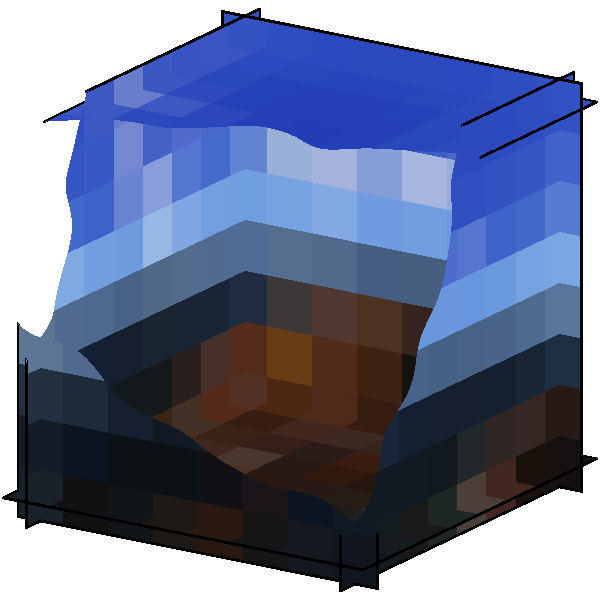
\includegraphics{figures/cube-nointerp.png} \hspace{1cm} 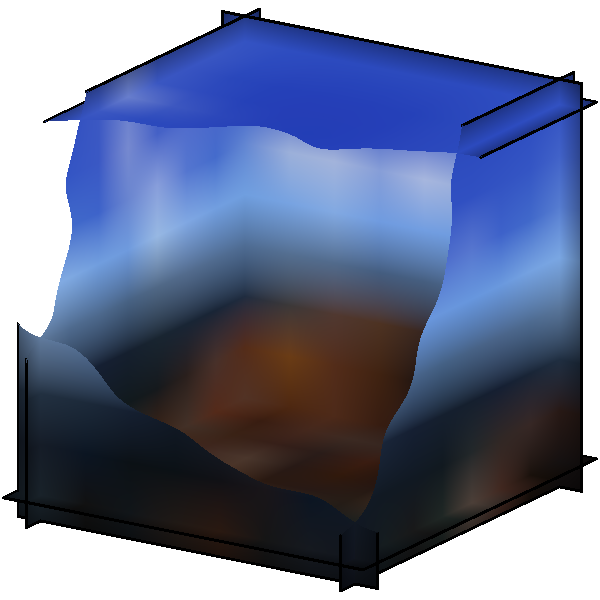
\includegraphics{figures/cube-interp.png}}
\caption{The face images protrude beyond the cube faces by half a pixel on each side to achieve seamless bilinear interpolation.}\label{fig:interpolation}
\end{figure}
Translating this into terms of field-of-view, one derives that for an image of width $w$ pixels, the field of view has to be
\begin{displaymath}
FOV = 2 \cdot \mathrm{atan} \frac{w}{w - 1}
\end{displaymath}
as sketched in figure~\ref{fig:fov}.
\begin{figure}[tbp]
\centering
\setlength{\fboxsep}{3mm}
\fbox{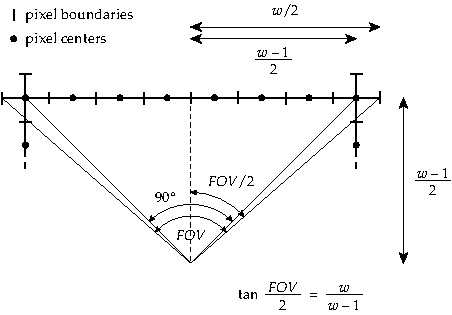
\includegraphics{figures/fov.pdf}}
\caption{Calculation of the field of view}\label{fig:fov}
\end{figure}
This expression is evaluated for some commonly used numbers in table~\ref{tab:fov}.
\begin{table}[htbp]
\centering
\begin{tabular}{cc}
\hline
\rule{0pt}{11pt}resolution [px] & FOV [\textdegree]\\[2pt]
\hline
\rule{0pt}{11pt}512 $\times$ 512 & 90.112\\
640 $\times$ 640 & 90.090\\
768 $\times$ 768 & 90.075\\
896 $\times$ 896 & 90.064\\
1024 $\times$ 1024 & 90.056\\[2pt]
\hline
\end{tabular}
\caption{Required field of view for commonly used cube face resolutions}\label{tab:fov}
\end{table}

\subsection{Patches}
\label{sec:patches}

A \emphindexed{patch} is an image that is placed on the (flat or panoramic) background at a specific location. You can programmatically show or hide patches, move them around, change their image, and modulate their colors (see section \secref{patchmethods}). To create a patch, add the following statement to \emph{node.lua}:
\hypertarget{patch}{}\ttindex{patch}\ttindex{face}\ttindex{x}\ttindex{y}\ttindex{w}\ttindex{h}\ttindex{visible}\ttindex{image}
\begin{Verbatim}[frame=single, framesep=1ex, xleftmargin=0.1\textwidth, xrightmargin=0.1\textwidth, commandchars=\\^\$]
patch {
  [face = \textit^face$,]
  x = \textit^x$ | nx = \textit^nx$,
  y = \textit^y$ | ny = \textit^ny$,
  [nz = \textit^nz$,]
  [w = \textit^width$ | nw = \textit^nw$,]
  [h = \textit^height$ | nh = \textit^nh$,]
  [anchorh = \textit^anchorh$,]
  [anchorv = \textit^anchorv$,]
  [angle = \textit^angle$,]
  [anglex = \textit^anglex$,]
  [angley = \textit^angley$,]
  [rotationorder = "xyz" | "yxz" | "zxy"
                 | "zyx" | "yzx" | "xzy",]
  [leftmargin = \textit^leftmargin$,]
  [rightmargin = \textit^rightmargin$,]
  [visible = \textit^visible$,]
  image = \textit^image$
}
\end{Verbatim}

The \verb|patch {|…\verb|}| statement returns a patch object that can be stored in a local variable for later reference (see section \secref{patchmethods}).

\minisec{Image}
\luaparam{image} is either a file name (see section \secref{specifyingpaths}) or an image object obtained from the \lualink{pipmak.getimage} or \lualink{pipmak.newimage} functions.
\luaparam{visible} is a boolean expression that specifies initial visibility of the patch, its default value is \texttt{true}.

For technical reasons (interpolation), the outermost pixels along each edge of a patch image should either be identical to the corresponding pixels of the background image or fully transparent. In other words, the patch image should be one pixel larger on each side than absolutely necessary. Otherwise, the patch may appear cut off along some edges.

\minisec{Basic Placement}
The \luaparam{face} parameter is only meaningful for cubic panoramas, it is a number from 1 to 6 that specifies the cube face on which the patch is to be placed. \luaparam{x} and \luaparam{y} are the coordinates of the anchor point of the patch image (see below; by default the top left corner) in pixels relative to the top left corner of the background image (or cube face). Width and height of the patch image are normally taken from the image file, but can optionally be specified by the \luaparam{w} and \luaparam{h} parameters (in pixels) to scale the image. In that case, \luaparam{leftmargin} and \luaparam{rightmargin} can be given to keep the leftmost and rightmost parts of the image at their original size and only stretch what's between them, similar to the way panels are scaled (see section \secref{panels}). By default, these parameters are 0, i.e.\ the whole image is scaled. Having rigid top and bottom margins is currently not possible.

\minisec{Rotation}
By giving an \luaparam{angle} in degrees different from the default 0, the patch is rotated counterclockwise. The center of rotation is given by the \luaparam{anchorh} and \luaparam{anchorv} parameters, which specify the horizontal and vertical coordinates of a point on the patch image in pixels from the top left corner. These are unscaled pixels, e.g.\ the center of a 20 pixels wide image is specified as \texttt{anchorh = 10} even if the image is being displayed at double the size by setting \texttt{w = 40}. By default, these parameters are 0, i.e.\ the anchor point is the top left corner. In addition to serving as the rotation center, the anchor point is also the point on the patch that is placed at the location specified by the \luaparam{x}, \luaparam{y} (see above) or \luaparam{nx}, \luaparam{ny}, \luaparam{nz} parameters (see below), as illustrated in figure~\ref{fig:patchplacement}.

\begin{figure}[tbb]
\centering
\setlength{\fboxsep}{3mm}
\rule{-10.01pt}{0pt}\fbox{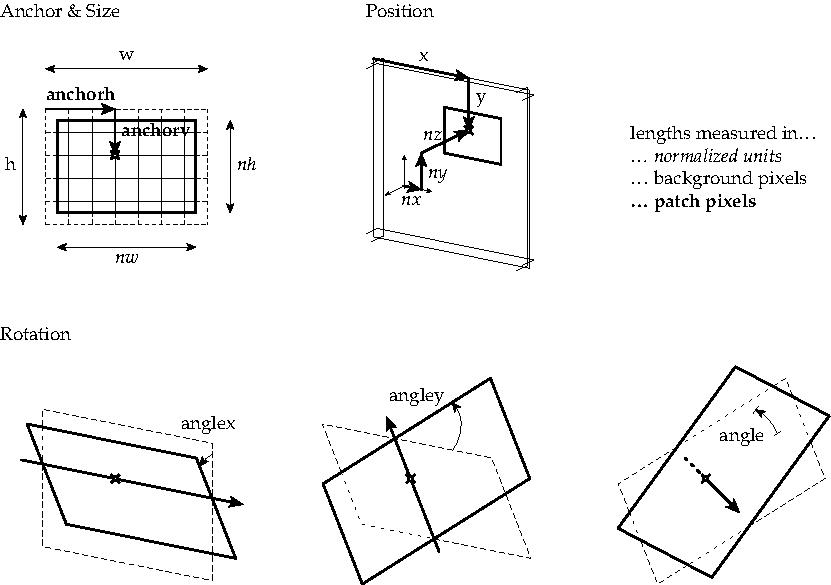
\includegraphics{figures/patch.pdf}}
\caption{Patch placement}\label{fig:patchplacement}
\end{figure}

\minisec{Advanced Placement in 3D}
Using the normalized coordinates \luaparam{nx}, \luaparam{ny}, \luaparam{nz} instead of \luaparam{x}, \luaparam{y}, a patch may be placed arbitrarily in 3 dimensions.

On cubic panoramas (where this is mainly useful), the normalized coordinate system is defined to have its origin at the center of the cube (i.e.\ the eye position), the \textit{x} axis in direction of face 2 (east), the \textit{y} axis in direction of face 5 (up), and the \textit{z} axis in direction of face 3 (south) (see figure~\ref{fig:facenumbers}). If a \luaparam{face} other than the default 1 is given (usually there is no need for this when using normalized coordinates), the coordinate system is rotated to have that face in direction $-z$. The cube faces are technically located at $\pm 1$ on each axis, but this is irrelevant, they can also be imagined infinitely far away.

On slides and panels, the \textit{x} and \textit{y} components of normalized coordinates are identical to the pixel coordinates used by the \luaparam{x} and \luaparam{y} parameters, and the \textit{z} axis points toward the viewer (but is irrelevant because the camera is orthographic).

After being grabbed by its anchor point and moved to the specified location, the patch is rotated around the anchor point in the following way, assuming that \luaparam{rotationorder} is at its default value of \texttt{"xyz"}, as illustrated in figure~\ref{fig:patchplacement}:
\begin{enumerate}
\item It starts out parallel to face 1 (or the given \luaparam{face}, if any), i.e.\ the \textit{xy} plane.
\item It is rotated around an axis parallel to its top and bottom edges, pointing to the right, by \luaparam{anglex} degrees.
\item It is rotated around an axis parallel to its (already rotated) left and right edges, pointing upward, by \luaparam{angley} degrees.
\item It is rotated in its (already rotated) plane, around an axis pointing inward, by \luaparam{angle} degrees.
\end{enumerate}
(Rotation directions are defined by the right-hand rule: point the thumb of your right hand in the direction of the rotation axis, then the other fingers curl in the direction of the rotation—e.g.\ step 2 moves the top edge inwards and the bottom edge outwards for positive angles.)

By setting \luaparam{rotationorder} to any of \texttt{"yxz"}, \texttt{"zxy"}, \texttt{"zyx"}, \texttt{"yzx"}, \texttt{"xzy"}, the order of these rotations can be changed. One particular application where an order different from the default \texttt{"xyz"} makes things much simpler is the following: to place a patch at azimuth \luaparam{az} and elevation \luaparam{el} on a panorama, facing the camera, use
\begin{Verbatim}[frame=single, framesep=1ex, xleftmargin=0.1\textwidth, xrightmargin=0.1\textwidth, commandchars=\\^\$]
nx = math.cos(math.rad(el))*math.sin(math.rad(az)),
ny = math.sin(math.rad(el)),
nz = -math.cos(math.rad(el))*math.cos(math.rad(az)),
rotationorder = "yxz",
angley = -az,
anglex = el
\end{Verbatim}

Width and height of the patch can also be specified in normalized units using the \luaparam{nw} and \luaparam{nh} parameters. Unlike \luaparam{w} and \luaparam{h}, which give the total width and height of the patch, these parameters describe the visible width and height. On panoramas and slides, this is one patch pixel less than the total width or height because a margin of half a pixel is cut off each side of the patch, so that the centers of the outermost pixels lie on the edge, to enable a bilinearly interpolated patch to blend seamlessly into a bilinearly interpolated background image. This is similar to what's done with the cube faces as described under “Making Cubic Panoramas” in section~\secref{makingcubicpanoramas}. As an example, this means that to make a patch of the same size coincide with cube face 1 (the same thing that would be accomplished by setting \texttt{face = 1, x = 0, y = 0}), you would specify \texttt{anchorh = 0.5, anchorv = 0.5, nx = -1, ny = 1, nz = -1, nw = 2, nh = 2}.

Note that although the normalized coordinates allow you to place patches geometrically behind each other, this has no influence on how they visibly overlap. All patches still overlap in the order of their definition, i.e.\ a patch defined further down in \emph{node.lua} will be seen in front of an earlier patch even if it is geometrically behind it.

\subsection{Controls}

Controls are invisible areas on the node background that can react to mouse actions (click, drag, enter, leave etc.). There are two types of controls, hotspots and handles. Hotspots are static and can have arbitrary shapes. The shape and location of hotspots is defined by an image file, the hotspot map, and their behavior is specified in the \emph{node.lua} file. Handles are rectangular, can be moved around, and have both shape and behavior defined in Lua code.

\subsubsection{Hotspot Maps}

To specify a hotspot map, write the following in \emph{node.lua}:
\hypertarget{hotspotmap}{}\ttindex{hotspotmap}
\begin{Verbatim}[frame=single, framesep=1ex, xleftmargin=0.1\textwidth, xrightmargin=0.1\textwidth, commandchars=\\^\$]
hotspotmap \textit^image$
\end{Verbatim}
\luaparam{image} is either a file name (see section \secref{specifyingpaths}) or an image object obtained from the \lualink{pipmak.getimage} function (in the latter case, it needs to be put in parentheses because Lua only allows the parentheses to be omitted around string literals). Hotspot maps are 256-color (indexed) images. Color index 0 means background, color index 1 is the first hotspot, index 2 the second etc. The actual colors don't matter, so you can use any color palette. A particularly suitable palette with easily distinguishable colors is included in the source distribution of Pipmak in \emph{hotspot-palette.gif} in the \emph{extras} folder. The hotspot map may contain more hotspots (colors) than are actually used, colors which don't have a corresponding \verb|hotspot {|…\verb|}| statement in \emph{node.lua} are ignored.

For slide and panel nodes, the image is stretched to cover the whole slide or panel (it need not have the same size or aspect ratio).

For panoramic nodes, the hotspot maps are equirectangular, that means that azimuth (0..360\textdegree) and elevation (-90\textdegree..90\textdegree) in the panorama are uniformly mapped to the horizontal and vertical axes in the image. The horizon in the panorama is mapped to the vertically centered horizontal line in the image, the point directly above the viewer (zenith) is stretched out along the whole top edge of the image, and correspondingly the point directly below (nadir) along the bottom edge. For example, if your hotspot map is $360 \times 180$ pixels, then the pixel at (68, 52) is what you see 38\textdegree\ ($= 90$\textdegree$\ -\ 52$\textdegree) above the horizon after you turn 68\textdegree\ to the right from the initial orientation.

See the \lualink{pipmak.saveequirect} function in section \secref{miscellaneous} for a preliminary hack to help you draw equirectangular hotspot maps.

\subsubsection{Hotspots and Handles}
\label{sec:hotspotsandhandles}

Controls can be specified in \emph{node.lua} in two different ways. Since controls are most commonly used to take the player to another node when clicked, a simplified syntax for this purpose is provided. For other purposes, such as buttons or sliders or other interactive elements, there is the extended syntax that allows complete control over the hotspot's or handle's behavior.

\minisec{Simplified Syntax for Navigational Controls}
\vspace{2ex}

\hypertarget{hotspot}{}\hypertarget{handle}{}\ttindex{hotspot}\ttindex{handle}\ttindex{x}\ttindex{y}\ttindex{az}\ttindex{el}\ttindex{w}\ttindex{h}\ttindex{target}\ttindex{effect}\ttindex{cursor}\ttindex{enabled}
\begin{Verbatim}[frame=single, framesep=1ex, xleftmargin=0.1\textwidth, xrightmargin=0.1\textwidth, commandchars=\\^\$]
hotspot | handle {
  [x = \textit^x$, y = \textit^y$,     \textit^--only for handles on flat$
  | cx = \textit^x$, cy = \textit^y$,] \textit^-- nodes$
  [az = \textit^az$, el = \textit^el$,     \textit^--only for handles on$
  | caz = \textit^az$, cel = \textit^el$,] \textit^-- panoramas$
  [w = \textit^width$, h = \textit^height$,] \textit^--only for handles$
  target = \textit^nodename$,
  [effect = \textit^function$,
  | effect = { \textit^function$, \textit^argument$, ... },]
  [cursor = \textit^cursor$,]
  [enabled = \textit^boolean$]
}
\end{Verbatim}
\luaparam{x} and \luaparam{y} specify the coordinates of the top left corner of the handle on slides and panels, in pixels relative to the top left corner of the node, while \luaparam{az} and \luaparam{el} do the same on panoramic nodes, in degrees (see figure~\ref{fig:facenumbers} for an illustration of the azimuth and elevation coordinates). Alternatively, you can specify the midpoint of the handle using \luaparam{cx} and \luaparam{cy} (flat) or \luaparam{caz} and \luaparam{cel} (panoramic). Width and height of the handle, in the same units, are specified by \luaparam{w} and \luaparam{h}. These properties only apply to handles, whereas all the others are valid for both handles and hotspots.

The \luaparam{target} property specifies the node name of the destination node. This is a path relative to the current node's parent folder, as explained in section \secref{specifyingpaths}—\linebreak simply the name of the other node if the two nodes lie in the same folder in the project.

The \luaparam{effect} property specifies the visual effect function from section \secref{transitioneffects} that is to be used. The value of this property is either a single function, which will be called without arguments (e.g. \lualink{pipmak.dissolve}, which is the default), or a list of a function and one or more arguments (e.g. \verb|{pipmak.wipe, pipmak.left, 1.5}|).

The \luaparam{cursor} property specifies the mouse cursor to be used while the mouse hovers over this control. It must either be one of the predefined constants listed in table~\ref{tab:cursors} on page \pageref{tab:cursors}, or a cursor object obtained from the \lualink{pipmak.loadcursor} function. By default, the node's standard cursor is used (or the global standard cursor if the node does not override it).

By setting the \luaparam{enabled} property to a boolean expression, a control can be conditionally enabled or disabled. Disabled controls are ignored by the mouse, they neither affect the cursor nor react to clicks and other mouse actions, as if they didn't exist at all. The default value is \texttt{true}, i.e.\ if this property is not specified, controls are enabled and work normally.

\minisec{Extended Syntax}
\vspace{2ex}

\ttindex{hotspot}\ttindex{handle}\ttindex{x}\ttindex{y}\ttindex{az}\ttindex{el}\ttindex{w}\ttindex{h}\ttindex{cursor}\ttindex{enabled}\ttindex{dont\_pan}\ttindex{onmouseup}\ttindex{onmousedown}\ttindex{onmouseenter}\ttindex{onmouseleave}\ttindex{onmousestilldown}\ttindex{omousewithin}\ttindex{onhilite}\ttindex{onenddrag}
\begin{Verbatim}[frame=single, framesep=1ex, xleftmargin=0.1\textwidth, xrightmargin=0.1\textwidth, commandchars=\\^\$]
hotspot | handle {
  [x = \textit^x$, y = \textit^y$,     \textit^--only for handles on flat$
  | cx = \textit^x$, cy = \textit^y$,] \textit^-- nodes$
  [az = \textit^az$, el = \textit^el$,     \textit^--only for handles on$
  | caz = \textit^az$, cel = \textit^el$,] \textit^-- panoramas$
  [w = \textit^width$, h = \textit^height$,] \textit^--only for handles$
  [cursor = \textit^cursor$,]
  [enabled = \textit^boolean$,]
  [dont_pan = \textit^boolean$,]
  [onmousedown = \textit^mousedownfunc$(\textit^self$),]
  [onmouseup = \textit^mouseupfunc$(\textit^self$),]
  [onmouseenter = \textit^mouseenterfunc$(\textit^self$),]
  [onmouseleave = \textit^mouseleavefunc$(\textit^self$),]
  [onmousestilldown = \textit^mousestilldownfunc$(\textit^self$),]
  [onmousewithin = \textit^mousewithinfunc$(\textit^self$),]
  [onhilite = \textit^hilitefunc$(\textit^self$, \textit^hilite$),]
  [onenddrag = \textit^enddragfunc$(\textit^self$)]
}
\end{Verbatim}

The \luaparam{x}, \luaparam{y}, \luaparam{az}, \luaparam{el}, \luaparam{cx}, \luaparam{cy}, \luaparam{caz}, \luaparam{cel}, \luaparam{w}, \luaparam{h}, \luaparam{cursor}, and \luaparam{enabled} properties are the same as discussed above for the simplified syntax.

The \hypertarget{dont\_pan}{\luaparam{dont\_pan}} property specifies whether the user is able to interact with this control by clicking and dragging. If it is \texttt{false}, dragging will pan the view instead of interacting with the control when the mouse is in joystick mode (see the \lualink{pipmak.setmousemode} function). Setting it to \texttt{true} will inhibit that behavior. By default, \luaparam{dont\_pan} is set to \texttt{true} for controls that have a \texttt{mousestilldown} handler and to \texttt{false} for those that don't. Set it explicitly to override the default value.

The \todo{document when they are called exactly} \luaparam{on...} properties specify event handler functions that are called when specific events occur on this control. They all receive the control that contains them as the first argument. The \texttt{hilite} handler in addition receives a second argument, a boolean that tells whether highlighting should be turned on or off.

Both the simple and the extended \verb|hotspot {|…\verb|}| and \verb|handle {|…\verb|}| statements return a control object that can be stored in a local variable for later reference (see section \secref{controlmethods}).


\subsection{Sounds}
\label{sec:sounds}
To create a sound source for playing a sound effect or a background loop, use either of the following statements in \emph{node.lua}:
\hypertarget{sound}{}\ttindex{sound}\ttindex{loop}\ttindex{volume}\ttindex{pitch}\ttindex{az}\ttindex{el}\ttindex{autoplay}
\begin{Verbatim}[frame=single, framesep=1ex, xleftmargin=0.1\textwidth, xrightmargin=0.1\textwidth, commandchars=\\^\$]
sound \textit^filename$
\end{Verbatim}
\begin{Verbatim}[frame=single, framesep=1ex, xleftmargin=0.1\textwidth, xrightmargin=0.1\textwidth, commandchars=\\^\$]
sound {
  \textit^filename$,
  [loop = \textit^boolean$,]
  [volume = \textit^volume$,]
  [pitch = \textit^pitch$,]
  [az = \textit^azimuth$, el = \textit^elevation$,]
  [autoplay = \textit^boolean$]
}
\end{Verbatim}

\luaparam{filename} is the file name (or path) of the Ogg Vorbis file to use (see section \secref{specifyingpaths}).

If \luaparam{loop} is \texttt{true}, the sound will play indefinitely once started, looping back to the beginning when it reaches the end. Otherwise (which is the default case), the sound will play once.

The \luaparam{volume}, a number between 0.0 (silent) and 1.0 (default volume), is multiplied to the volume (amplitude) of the sound.

The \luaparam{pitch} number is multiplied to the speed at which the sound is played, changing its pitch. The default value is 1.0. Multiply or divide by 2 to raise or lower the pitch by one octave, multiply by \texttt{math.pow(2, 1/12)} to raise by one (tempered) semitone, etc.

\luaparam{az} and \luaparam{el} specify the direction from which the sound originates on a panorama (azimuth and elevation in degrees, see figure~\ref{fig:facenumbers}). By default, sounds are omnidirectional (play on all channels, independent of the player’s orientation). Directional sound only works for mono sound files, stereo sounds are always played without adjusting their channel distribution to the viewing direction.

If \luaparam{autoplay} is \texttt{true}, the sound automatically starts playing when the node is entered and stops when the node is left. This is usually used together with \texttt{loop = true} for background sounds that are specific to one node (obviously, it is not suitable for background sounds that need to continue playing seamlessly over node transitions).

The \verb|sound {|…\verb|}| statement returns a sound object, which you will usually (unless you are using \luaparam{autoplay}) assign to a local or global variable to play it or change its properties later (see section \secref{soundmethods}), e.g.
\begin{Verbatim}[frame=single, framesep=1ex, xleftmargin=0.1\textwidth, xrightmargin=0.1\textwidth, commandchars=\\^\$]
local myeffect = sound "effect.ogg"
myambient = sound { "background.ogg", loop = true }

hotspot {
  onmousedown = function() myeffect:play() end
}
\end{Verbatim}


\subsection{Keyboard Handling}
Pipmak projects can react to key presses. To register a function as a \ttindexed{keydown} handler, use
\hypertarget{onkeydown}{}\ttindex{onkeydown}
\begin{Verbatim}[frame=single, framesep=1ex, xleftmargin=0.1\textwidth, xrightmargin=0.1\textwidth, commandchars=\\^\$]
onkeydown (\textit^keydownfunc$(\textit^key$ [, \textit^char$]))
\end{Verbatim}
Placing this code in \emph{node.lua} creates a \emph{local} \texttt{keydown} handler for the corresponding node. Placing it in \emph{main.lua} creates a \emph{global} \texttt{keydown} handler. When a key is pressed, Pipmak calls the local \texttt{keydown} handler of the topmost displayed node (if it has one). If this handler returns \texttt{true}, indicating that it handled the key press event, processing stops. If it returns \texttt{false} (or nothing), indicating that it isn't interested in the key press event, the local \texttt{keydown} handler of the next node is called, and so on. The event is thus passed down the stack of all displayed nodes, until either it is handled (a handler returns \texttt{true}), or it reaches the bottom (none of the displayed nodes were interested). In the latter case, the global \texttt{keydown} handler is finally called.

Information about which key was pressed is passed to the \texttt{keydown} handlers as a numerical code in \luaparam{key}. For keys that generate characters, the code is the ASCII code of the character, which can be determined using the \texttt{string.byte()} function (e.g. \texttt{string.byte( "a")} returns 97, which is the key code of the A key). For other keys, Pipmak supplies a range of predefined constants in the \texttt{pipmak} table (\verb|pipmak.key_|…), listed in table~\ref{tab:keys}.

\begin{table}[htbp]
\centering
\begin{tabular}{cccc}
\hline
\rule{0pt}{11pt}\begin{tabular}[t]{@{}l@{}}
\luaconstantshort{pipmak}{key\_backspace}\\
\luaconstantshort{pipmak}{key\_tab}\\
\luaconstantshort{pipmak}{key\_clear}\\
\luaconstantshort{pipmak}{key\_return}\\
\luaconstantshort{pipmak}{key\_pause}\\
\luaconstantshort{pipmak}{key\_esc}\\
\luaconstantshort{pipmak}{key\_delete}\\
\luaconstantshort{pipmak}{key\_kp\_0}\\
\luaconstantshort{pipmak}{key\_kp\_1}\\
\luaconstantshort{pipmak}{key\_kp\_2}\\
\luaconstantshort{pipmak}{key\_kp\_3}\\
\luaconstantshort{pipmak}{key\_kp\_4}\\
\end{tabular}
&
\begin{tabular}[t]{@{}l@{}}
\luaconstantshort{pipmak}{key\_kp\_5}\\
\luaconstantshort{pipmak}{key\_kp\_6}\\
\luaconstantshort{pipmak}{key\_kp\_7}\\
\luaconstantshort{pipmak}{key\_kp\_8}\\
\luaconstantshort{pipmak}{key\_kp\_9}\\
\luaconstantshort{pipmak}{key\_kp\_period}\\
\luaconstantshort{pipmak}{key\_kp\_divide}\\
\luaconstantshort{pipmak}{key\_kp\_multiply}\\
\luaconstantshort{pipmak}{key\_kp\_minus}\\
\luaconstantshort{pipmak}{key\_kp\_plus}\\
\luaconstantshort{pipmak}{key\_kp\_enter}\\
\luaconstantshort{pipmak}{key\_kp\_equals}\\
\end{tabular}
&
\begin{tabular}[t]{@{}l@{}}
\luaconstantshort{pipmak}{key\_arrow\_up}\\
\luaconstantshort{pipmak}{key\_arrow\_down}\\
\luaconstantshort{pipmak}{key\_arrow\_right}\\
\luaconstantshort{pipmak}{key\_arrow\_left}\\
\luaconstantshort{pipmak}{key\_insert}\\
\luaconstantshort{pipmak}{key\_home}\\
\luaconstantshort{pipmak}{key\_end}\\
\luaconstantshort{pipmak}{key\_pageup}\\
\luaconstantshort{pipmak}{key\_pagedown}\\
\luaconstantshort{pipmak}{key\_f1}\\
\luaconstantshort{pipmak}{key\_f2}\\
\luaconstantshort{pipmak}{key\_f3}\\
\end{tabular}
&
\begin{tabular}[t]{@{}l@{}}
\luaconstantshort{pipmak}{key\_f4}\\
\luaconstantshort{pipmak}{key\_f5}\\
\luaconstantshort{pipmak}{key\_f6}\\
\luaconstantshort{pipmak}{key\_f7}\\
\luaconstantshort{pipmak}{key\_f8}\\
\luaconstantshort{pipmak}{key\_f9}\\
\luaconstantshort{pipmak}{key\_f10}\\
\luaconstantshort{pipmak}{key\_f11}\\
\luaconstantshort{pipmak}{key\_f12}\\
\luaconstantshort{pipmak}{key\_f13}\\
\luaconstantshort{pipmak}{key\_f14}\\
\luaconstantshort{pipmak}{key\_f15}\\
\end{tabular}
\vspace{3pt}\\
\hline
\end{tabular}
\caption{Keyboard constants in the \texttt{pipmak} table}\label{tab:keys}
\end{table}

The second argument \luaparam{char} to the \texttt{keydown} handler contains the character that would be generated by the key press, if any (e.g. if the A key is pressed, \luaparam{char} may be \texttt{"a"} or \texttt{"A"} depending on whether the shift key was held down). It is encoded in UTF-8, meaning that it may be more than one byte.

Here is an example of a local \texttt{keydown} handler:
\begin{Verbatim}[frame=single, framesep=1ex, xleftmargin=0.1\textwidth, xrightmargin=0.1\textwidth, commandchars=\\^\$]
onkeydown (
  function(key)
    if key == string.byte(" ") then
      pipmak.print("You pressed the space bar!")
      return true
    elseif key == pipmak.key_return then
      pipmak.print("You pressed the return key!")
      return true
    else
      return false
    end
  end
)
\end{Verbatim}

Handling of Pipmak's default keys (such as ESC to bring up the main menu) is done by the default global \texttt{keydown} handler. This means that you have to provide these functions yourself if you choose to set your own global \texttt{keydown} handler. Have a look at \emph{defaults.lua} in Pipmak's resources (inside the application bundle or in an external ZIP file, depending on your OS) to see how it is done.

\section{Scripting}
\label{sec:scripting}

Scripting in Pipmak is done in Lua, a simple and powerful embeddable scripting language. To find out more about Lua, visit \url{http://www.lua.org/} (especially the “community” and “documentation” sections). An essential resource for Lua programming is the Lua reference manual: \url{http://www.lua.org/manual/5.0/}.

Pipmak provides a complete Lua 5.0 environment including the \emph{base}, \emph{string}, \emph{table}, and \emph{math} standard libraries as well as the \emph{pack} extension (which is internally used for saving games). In addition, it defines numerous functions for interaction with the game engine. Most of these are provided in the global table \texttt{pipmak} and are discussed in the following sections.

\subsection{Storing Game State}
\label{sec:storinggamestate}

To keep track of the state of your game world, you should use the global table \hypertarget{state}{\ttindexed{state}}, which is predefined by Pipmak. The contents of this table are included in saved game files. You can use arbitrary strings, numbers, booleans, or tables as keys and values in \ttindexed{state}. Don't use global variables outside of \ttindexed{state} for state storage, as they are not saved and restored when saving games and loading saved games.

\subsection{Navigation}
\label{sec:navigation}
\luafunction{pipmak}{gotonode}{nodename [, inbackground]}
\luadescription{Go to node \luaparam{nodename}. \luaparam{nodename} is a path relative to the current node's parent folder, as explained in section \secref{specifyingpaths}—simply the name of the other node if the two nodes lie in the same folder in the project.

By default, the transition is accompanied by a 0.5 second dissolve effect, but you can specify a different effect by calling one of the functions from section \secref{transitioneffects} immediately before this function.

If \luaparam{inbackground} is \texttt{true}, the new node replaces the background node\index{background node}, otherwise it replaces the node from which the function is called (as defined by the \lualink{pipmak.thisnode} function). (Obviously this only matters if you are calling the function from an overlay, see section \secref{thenodestack}.)}

\subsection{Transition Effects}
\label{sec:transitioneffects}
\index{transition effect}
Using the following functions, any visual change on your screen can be adorned by a transition effect. Most often, this is used for node transitions, but it can occasionally be useful for other changes, like fading patches in and out.

The transition effect happens between the state of the screen at the time the effect function was called and the state after the return from Lua (recall that the screen is never updated while any Lua code is running). In other words, call the effect function immediately before you do your changes to the screen (go to a different node, show or change a patch, etc.). It will capture the “old image” (without displaying it), and the transition to the “new image” will begin as soon as your Lua code returns.
\vspace{2ex}

\luafunction{pipmak}{dissolve}{[scale [, duration]]}
\luadescription{A smooth fade between the old and the new image. If a \luaparam{scale} factor different from 1 (the default) is given, the old image is gradually zoomed in to that factor while it fades out. \luaparam{duration} is in seconds, the default is 0.5.}
\luafunction{pipmak}{rotate}{direction [, angle [, duration]]}
\luadescription{The old image is shifted out in \luaparam{direction} while the new image slides in from the opposite side. \luaparam{direction} is one of \luaconstant{pipmak}{left}, \luaconstant{pipmak}{right}, \luaconstant{pipmak}{up}, \luaconstant{pipmak}{down}. If an \luaparam{angle} different from 0 (the default) is given, a rotation of the viewer by \luaparam{angle} degrees is simulated. Negative angles give the “rotating cube” effect known from Apple's Keynote or Mac OS X's fast user switching. \luaparam{duration} is in seconds, the default is 0.5.}
\luafunction{pipmak}{wipe}{direction [, duration]}
\luadescription{The new image is revealed along a boundary moving in \luaparam{direction}. Neither of the images moves. \luaparam{direction} is one of \luaconstant{pipmak}{left}, \luaconstant{pipmak}{right}, \luaconstant{pipmak}{up}, \luaconstant{pipmak}{down}. \luaparam{duration} is in seconds, the default is 0.5.}

To get an abrupt transition without any effect, use any of these functions with a \luaparam{duration} of 0.

\subsection{Mouse Cursors}
\label{sec:mousecursors}
\index{cursor}Pipmak offers a variety of built-in cursors, listed in table~\ref{tab:cursors}. You can also define your own cursors using the \lualink{pipmak.loadcursor} function.
\begin{table}[htbp]
\centering
\begin{tabular}{c@{\hspace{1cm}}c}
\hline
\begin{tabular}[t]{@{}ll@{}}
\rule{0pt}{15pt}\raisebox{-8bp}{
\includegraphics[viewport = -1 0 19 20]{../resources/resources/cursor_hand.png}} & \luaconstant{pipmak}{hand}\\
\rule{0pt}{15pt}\raisebox{-8bp}{
\includegraphics[viewport = -1 0 19 20]{../resources/resources/cursor_hand_open.png}} & \luaconstant{pipmak}{hand\_open}\\
\rule{0pt}{15pt}\raisebox{-8bp}{
\includegraphics[viewport = -3 -1 17 19]{../resources/resources/cursor_hand_closed.png}} & \luaconstant{pipmak}{hand\_closed}\\
\rule{0pt}{15pt}\raisebox{-8bp}{
\includegraphics[viewport = -1 -1 19 19]{../resources/resources/cursor_hand_left.png}} & \luaconstant{pipmak}{hand\_left}\\
\rule{0pt}{15pt}\raisebox{-8bp}{
\includegraphics[viewport = -1 -1 19 19]{../resources/resources/cursor_hand_right.png}} & \luaconstant{pipmak}{hand\_right}\\
\rule{0pt}{15pt}\raisebox{-8bp}{
\includegraphics[viewport = -1 -1 19 19]{../resources/resources/cursor_hand_lleft.png}} & \luaconstant{pipmak}{hand\_lleft}\\
\rule{0pt}{15pt}\raisebox{-8bp}{
\includegraphics[viewport = -1 -1 19 19]{../resources/resources/cursor_hand_rright.png}} & \luaconstant{pipmak}{hand\_rright}\\
\rule{0pt}{15pt}\raisebox{-8bp}{
\includegraphics[viewport = -3 0 17 20]{../resources/resources/cursor_hand_up.png}} & \luaconstant{pipmak}{hand\_up}\\
\rule{0pt}{15pt}\raisebox{-8bp}{
\includegraphics[viewport = -3 0 17 20]{../resources/resources/cursor_hand_down.png}} & \luaconstant{pipmak}{hand\_down}\\
\rule{0pt}{15pt}\raisebox{-8bp}{
\includegraphics[viewport = -1 0 19 20]{../resources/resources/cursor_hand_forward.png}} & \luaconstant{pipmak}{hand\_forward}\\
\rule{0pt}{15pt}\raisebox{-8bp}{
\includegraphics[viewport = -1 0 19 20]{../resources/resources/cursor_hand_back.png}} & \luaconstant{pipmak}{hand\_back}\\
\rule{0pt}{15pt}\raisebox{-8bp}{
\includegraphics[viewport = -1 -2 19 18]{../resources/resources/cursor_hand_lout.png}} & \luaconstant{pipmak}{hand\_lout}\\[7bp]
\end{tabular}
&
\begin{tabular}[t]{@{}ll@{}}
\rule{0pt}{15pt}\raisebox{-8bp}{
\includegraphics[viewport = -1 -2 19 18]{../resources/resources/cursor_hand_rout.png}} & \luaconstant{pipmak}{hand\_rout}\\
\rule{0pt}{15pt}\raisebox{-10bp}{
\includegraphics[viewport = 2 0 22 24]{../resources/resources/cursor_hand_zoom.png}} & \luaconstant{pipmak}{hand\_zoom}\\
\rule{0pt}{15pt}\raisebox{-10bp}{
\includegraphics[viewport = 2 0 22 24]{../resources/resources/cursor_hand_zoomin.png}} & \luaconstant{pipmak}{hand\_zoomin}\\
\rule{0pt}{15pt}\raisebox{-10bp}{
\includegraphics[viewport = 2 0 22 24]{../resources/resources/cursor_hand_zoomout.png}} & \luaconstant{pipmak}{hand\_zoomout}\\
\rule{0pt}{15pt}\raisebox{-8bp}{
\includegraphics[viewport = -1 0 19 20]{../resources/resources/cursor_zip.png}} & \luaconstant{pipmak}{zip}\\
\rule{0pt}{15pt}\raisebox{-8bp}{
\includegraphics[viewport = -3 0 17 20]{../resources/resources/cursor_arrow.png}} & \luaconstant{pipmak}{arrow}\\
\rule{0pt}{15pt}\raisebox{-8bp}{
\includegraphics[viewport = -4 -3 16 17]{../resources/resources/cursor_pencil.png}} & \luaconstant{pipmak}{pencil}\\
\rule{0pt}{15pt}\raisebox{-8bp}{
\includegraphics[viewport = -1 -2 19 18]{../resources/resources/cursor_eyedropper.png}} & \luaconstant{pipmak}{eyedropper}\\
\rule{0pt}{15pt}\raisebox{-8bp}{
\includegraphics[viewport = 0 0 20 20]{../resources/resources/cursor_pan.png}} & \luaconstant{pipmak}{pan}\\
\rule{0pt}{15pt}\raisebox{-8bp}{
\includegraphics[viewport = -5 -5 15 15]{../resources/resources/cursor_dot.png}} & \luaconstant{pipmak}{dot}\\
\rule{0pt}{15pt}\raisebox{-8bp}{
\includegraphics[viewport = 0 -3 20 17]{../resources/resources/cursor_triangle.png}} & \luaconstant{pipmak}{triangle}\\[7bp]
\end{tabular}\\
\hline
\end{tabular}
\caption{Predefined mouse cursors}\label{tab:cursors}
\end{table}

Which cursor is used at a particular time can be influenced on four levels, where the more specific levels take precedence over the more general ones:
\begin{itemize}
\item There is a global standard cursor that is used whenever none of the other levels override it. By default, this is the hand cursor, but you can change it using the \lualink{pipmak.setstandardcursor} function.
\item A node can have a standard cursor that overrides the global standard cursor on that particular node. This is specified by the \luaparam{cursor} property in the \lualink{slide}, \lualink{panel}, or \lualink{cubic} statement, or by calling the \luamethodlink{node}{setstandardcursor} method of the node.
\item A control (\lualink{hotspot} or \lualink{handle}) can have a cursor that is used when the mouse is within that control.
\item At any time, you can change the cursor by calling the \lualink{pipmak.setcursor} function. The new cursor will be used as long as the mouse stays within the same control and node (or until you call the function again with a different cursor). Entering or leaving a control or a node will reset the cursor to the corresponding standard cursor.
\end{itemize}

\luafunction{pipmak}{loadcursor}{filename, hotx, hoty}
\luadescription{Loads the image file \luaparam{filename} (see section \secref{specifyingpaths}) and returns a cursor object that can be used wherever cursors are expected. (\luaparam{hotx}, \luaparam{hoty}) are the coordinates of (the top left corner of) the cursor's active pixel (also called “hotspot”, but not to be confused with \hyperlink{hotspot}{Pipmak's hotspots}) in pixels relative to the top left corner of the image.

This function is typically called in \hyperlink{onopenproject}{\texttt{openproject}} handlers to load cursors that are used throughout the project and assign them to global variables, or in \hyperlink{onenternode}{\texttt{enternode}} handlers if the cursor is only used on one node.}
\luafunction{pipmak}{setstandardcursor}{cursor}
\luadescription{Sets the global standard cursor that is used whenever nodes or controls don't specify their own cursors to \luaparam{cursor}, which must either be one of the predefined constants listed in table~\ref{tab:cursors} on page \pageref{tab:cursors}, or a cursor object obtained from the \lualink{pipmak.loadcursor} function.

This function is typically called in the \hyperlink{onopenproject}{\texttt{openproject}} handler after loading a custom standard cursor.}
\luafunction{pipmak}{setcursor}{cursor}
\luadescription{Temporarily sets the mouse cursor to \luaparam{cursor}, which must either be one of the predefined constants listed in table~\ref{tab:cursors} on page \pageref{tab:cursors}, or a cursor object obtained from the \lualink{pipmak.loadcursor} function. Entering or leaving a control or another node with the mouse will reset the cursor to the control's or node's standard cursor.}

\subsection{Miscellaneous Engine State}

\luafunction{pipmak}{clickloc}{}
\luadescription{Returns two values, the coordinates of the last “mouse down” event in the coordinate system of the node on which it happened (x and y in pixels relative to the top left corner on flat nodes, azimuth and elevation in degrees on panoramas).}
\luafunction{pipmak}{mouseloc}{}
\luadescription{Returns two values, the coordinates of the mouse pointer in the coordinate system of the current node.}
\luafunction{pipmak}{mouseminusclickloc}{}
\luadescription{This convenience function is equivalent to what could be written as \texttt{\lualink{pipmak.mouseloc}() - \lualink{pipmak.clickloc}()} if Lua had a “vectorized” subtraction operator, i.e.\ it returns by how much the mouse has moved since the mouse button was pressed.}
\luafunction{pipmak}{mouseisdown}{}
\luadescription{Returns \texttt{true} if the (left) mouse button is down, \texttt{false} if it is up.}
\luafunction{pipmak}{pushmousemode}{mode}
\luadescription{Changes the current mouse mode to \luaparam{mode} (which must be either \luaconstant{pipmak}{joystick} or \luaconstant{pipmak}{direct}, see \lualink{pipmak.setmousemode}). This function is meant for temporary changes that are undone later, in contrast to \lualink{pipmak.setmousemode}, which permanently sets the standard mouse mode. These temporary mouse modes are maintained on a stack, where the topmost entry determines the mode that is currently used. This function places a new entry with the given mode on top of the stack. Returns a token that must be stored and later passed to \lualink{pipmak.popmousemode} to remove the entry from the stack. See also the \lualink{mousemode} property of nodes.}
\luafunction{pipmak}{popmousemode}{token}
\luadescription{Undoes the mouse mode change indentified by \luaparam{token}, which was obtained from \lualink{pipmak.pushmousemode}, by removing the corresponding entry from the stack of temporary mouse modes. If this entry was at the top of the stack, the mouse mode returns to the entry below it, otherwise the entry is just withdrawn from the stack without immediate effect\footnote{In other words, mouse modes can be popped in any order, not just the reverse of the order in which they were pushed, so this isn't strictly a “pop” operation in the usual sense.}. The standard mouse mode, set by \lualink{pipmak.setmousemode}, is always at the bottom of the stack. Returns \texttt{true} if the removal was successful and \texttt{false} if \luaparam{token} was invalid (e.g.\  because it has already been popped before).}
\luafunction{pipmak}{getcurrentnode}{}
\luadescription{Returns the name of the current background node. Equivalent to \texttt{\lualink{pipmak.backgroundnode}():\luamethodlink{node}{getname}()}.}
\luafunction{pipmak}{setviewdirection}{azimuth, elevation}
\luadescription{Sets the current viewing direction on panoramic nodes. The viewing direction is a global state, you may also set it while on an non-panoramic node, although the effect will only be visible the next time you enter a panoramic node.}
\luafunction{pipmak}{getviewdirection}{}
\luadescription{Returns azimuth and elevation of the current viewing direction on panoramic nodes.}


\subsection{Nodes}
\label{sec:nodemethods}

\subsubsection{The Node Stack}
\label{sec:thenodestack}
At any time, Pipmak displays one or more nodes in a defined stacking order. If a node doesn't cover the whole screen or has transparent regions, nodes lower in the stack will show through. The node at the bottom of the stack is called the \emphindexed{background node}. All the other nodes, if there are any, are referred to as \emph{overlays}\index{overlay}. To change the background node, use the \lualink{pipmak.gotonode} function. To add a new overlay or to bring an existing overlay to the front, use the \lualink{pipmak.overlaynode} function. To remove an overlay, call its \luamethodlink{node}{closeoverlay} method.

\subsubsection{Inter-Node Communication}
\label{sec:internodecommunication}
Often some way of communication between two or more simultaneously displayed nodes is needed. The obvious naive way of achieving this would be defining a global function in node A and calling it from node B. However, this doesn't work as expected in many cases: Lua doesn't care in which file a function was defined. Even if it was defined in the \emph{node.lua} file of node A, calling the function from node B will make the code run in node B. Anything it does that makes an implicit assumption about the “current node” will affect node B, not node A.

To solve this problem, a messaging system is provided. By including
\hypertarget{messages}{}\ttindex{messages}
\begin{Verbatim}[frame=single, framesep=1ex, xleftmargin=0.1\textwidth, xrightmargin=0.1\textwidth, commandchars=\\^\$]
messages {
  \textit^messagename$ = \textit^handler$,
  ...
}
\end{Verbatim}
in its \emph{node.lua}, a node can define a set of messages to which it responds. Each entry in the messages table links a string \luaparam{messagename} to a \luaparam{handler} function that will be called when the corresponding message is received. The message handler function then runs in the node where it was defined, not in the one who sent the message. To send a message to a node, use its \luamethodlink{node}{message} method.

\subsubsection{Node Objects}
\label{sec:nodeobjects}
Every node that is being displayed by Pipmak is represented in Lua by a node object. Node objects are only valid as long as the corresponding node is being displayed. Leaving and re-entering a node will create a new node object, the old object will remain invalid. There are several ways of getting hold of these objects to programmatically manipulate them:
\vspace{2ex}

\luafunction{pipmak}{overlaynode}{nodeid [, dontsave]}
\luadescription{Loads node number \luaparam{nodeid} and displays it as an overlay\index{overlay} on top of all other currently visible nodes. If the node is already being displayed as an overlay, brings it to the front. This means that it is not possible to display more than one instance of the same node as overlays simultaneously. It is, however, possible to display the same node as the background node and as an overlay at the same time.

If \luaparam{dontsave} is \texttt{true}, the overlay will not be included in saved game files. This is useful e.g.\ for a menu panel with a “save game” button—opening a saved game should return directly to the game, not to that panel.

Returns the newly displayed node.}
\luafunction{pipmak}{thisnode}{}
\luadescription{Returns the node in whose code this function is called. This may not necessarily be the node in whose \emph{node.lua} the code sits, since Lua code is free to call functions defined in any other Lua file. It is the node from which the current call into Lua originated.}
\luafunction{pipmak}{backgroundnode}{}
\luadescription{Returns the current background node.}

All node objects have the following methods:
\vspace{2ex}

\luamethod{node}{getname}{}
\luadescription{Returns \luaparam{node}'s name. This is the full path of the node folder from the top level of the project, without a leading \texttt{/} (i.e.\ for the usual case of a node located at the top level of the project, simply the folder name). See also section \secref{specifyingpaths}.}
\luamethod{node}{getid}{}
\luadescription{\emph{This method is deprecated and will be removed in a future version.} An alternative name for the \luamethodlink{node}{getname} method, provided for backwards compatibility.}
\luamethod{node}{setstandardcursor}{cursor}
\luadescription{Sets the mouse cursor to be used on \luaparam{node} instead of the global standard cursor (see section \secref{mousecursors}). \luaparam{cursor} must either be one of the predefined constants listed in table~\ref{tab:cursors} on page \pageref{tab:cursors}, or a cursor object obtained from the \lualink{pipmak.loadcursor} function.}
\luamethod{node}{closeoverlay}{}
\luadescription{If \luaparam{node} is being displayed as an overlay\index{overlay}, leave it and remove it from the stack of displayed nodes. Calling this method on the background node has no effect.}
\luamethod{node}{message}{message [, arguments, ...]}
\luadescription{Send \luaparam{message} to \luaparam{node}, passing \luaparam{arguments} to the message handler. Waits for the message handler to complete and returns whatever the message handler returns. If \luaparam{node} has no handler for \luaparam{message}, does nothing and returns nothing. See section \secref{internodecommunication}.}

In addition to the methods above, panel nodes have the following methods:
\vspace{2ex}

\luamethod{panel}{moveto}{relx [, rely [, absx [, absy [, duration]]]]}
\luadescription{Sets the relative and absolute components of the position of \luaparam{panel}. Any of \luaparam{relx}, \luaparam{rely}, \luaparam{absx}, \luaparam{absy} may be \texttt{nil} (or omitted, if no other parameters follow it). See section \secref{panels} for an explanation of these parameters and their default values. If a \luaparam{duration} in seconds greater than 0 is given, the movement is not instantaneous but animated. Animation happens asynchronously, that is, the method returns immediately and does not wait for the animation to complete (which would be pointless because the screen is not updated while any Lua code is running).}
\luamethod{panel}{moveby}{dx, dy}
\luadescription{Moves \luaparam{panel} by (\luaparam{dx}, \luaparam{dy}) pixels. Tries to be smart about adjusting both the relative and the absolute component of the position in such a way that the panel moves in a sensible manner when the Pipmak window is resized (or the screen resolution changes, in fullscreen mode). This provides an easy way of making a panel draggable: use a control with}
\begin{Verbatim}[frame=single, framesep=1ex, xleftmargin=0.2\textwidth, xrightmargin=0.1\textwidth, commandchars=\\^\$]
onmousestilldown = function()
  pipmak.thisnode():moveby(pipmak.
    mouseminusclickloc())
end
\end{Verbatim}
\luamethod{panel}{location}{}
\luadescription{Returns the relative and absolute components of the location of \luaparam{panel}, in the order \emph{relx}, \emph{rely}, \emph{absx}, \emph{absy}. See \lualink{panel:moveto} and section \secref{panels} for an explanation of the meaning of these values.}


\subsection{Patches}
\label{sec:patchmethods}

There are two ways of getting hold of a patch to programmatically manipulate it: Either store a reference to it when a patch is created,
\begin{Verbatim}[frame=single, framesep=1ex, xleftmargin=0.1\textwidth, xrightmargin=0.1\textwidth, commandchars=\\^\$]
local mypatch = \lualink^patch$ { ... }
\end{Verbatim}
or use the \lualink{pipmak.getpatch} function:
\vspace{2ex}

\luafunction{pipmak}{getpatch}{patchid}
\luadescription{Returns patch number \luaparam{patchid} of the current node, or \texttt{nil} if there's no such patch in the current node. Patches are numbered starting from 1 in the order of their creation. See the \lualink{pipmak.thisnode} function for a definition of what the “current node” is.}

Patch objects are only valid as long as the node that contains them is displayed. They have the following methods:
\vspace{2ex}

\luamethod{patch}{getid}{}
\luadescription{Returns \luaparam{patch}'s identification number. Patches are numbered starting from 1 in the order of their creation. (\texttt{pipmak.getpatch(i):getid() == i} for all \texttt{i} from 1 to the number of patches of the current node.)}
\luamethod{patch}{location}{}
\luadescription{Returns three values: the x and y coordinates of \luaparam{patch} and its face number. See \lualink{patch:moveto}.}
\luamethod{patch}{moveto}{x, y [, face]}
\luadescription{Sets the coordinates of \luaparam{patch}'s anchor point (the top left left corner, by default) in pixels relative to the top left corner of the background image to (\luaparam{x}, \luaparam{y}) on cube face number \luaparam{face} (1–6). If \luaparam{face} is omitted, the patch is left on its current face. On flat nodes, \luaparam{face} is meaningless.}
\luamethod{patch}{move}{properties}
\luadescription{Updates any of the positional properties of \luaparam{patch} to the values given in the table \luaparam{properties}. Settable properties are \texttt{face}, \texttt{x}, \texttt{y}, \texttt{nx}, \texttt{ny}, \texttt{nz}, \texttt{w}, \texttt{h}, \texttt{nw}, \texttt{nh}, \texttt{anchorh}, \texttt{anchorv}, \texttt{angle}, \texttt{anglex}, \texttt{angley}, as defined in section \secref{patches}. E.g.\ rotating a patch to 60\textdegree\ is achieved by \texttt{patch:move\{angle = 60\}}, and \texttt{patch:moveto(16, 28)} is equivalent to \texttt{patch:move\{x = 16, y = 28\}}.}
\luamethod{patch}{isvisible}{}
\luadescription{Returns \texttt{true} if \luaparam{patch} is visible and \texttt{false} otherwise.}
\luamethod{patch}{setvisible}{v}
\luadescription{Shows or hides \luaparam{patch} depending on whether the boolean value of \luaparam{v} is \texttt{true} or \texttt{false}.}
\luamethod{patch}{setimage}{image}
\luadescription{Set \luaparam{patch}'s image to \luaparam{image}, which is either a file name (see section \secref{specifyingpaths}) or an image object obtained from the \lualink{pipmak.getimage} or \lualink{pipmak.newimage} functions.}
\luamethod{patch}{getcolor}{}
\luadescription{Returns four values: the red, green, blue, and alpha components of \luaparam{patch}'s color. See \lualink{patch:setcolor}.}
\luamethod{patch}{setcolor}{red, green, blue [, alpha]}
\luadescription{Sets \luaparam{patch}'s color to (\luaparam{red}, \luaparam{green}, \luaparam{blue}) and its opacity to \luaparam{alpha} (if omitted, opacity is left unchanged). All components range from 0.0 to 1.0.

Before a patch is displayed, its pixel values are multiplied by the color values set by this function. Examples: \texttt{p:setcolor(1, 1, 1, 1)} makes the patch appear in its normal colors (which is the default for newly created patches), \texttt{p:setcolor(0, 0, 0, 1)} makes it black, \texttt{p:setcolor(0, 1, 0, 1)} only leaves the green component, and \texttt{p:setcolor(1, 1, 1, 0.5)} makes it half-transparent.}
\luamethod{patch}{getalpha}{}
\luadescription{Returns \luaparam{patch}'s alpha (opacity) value. See \lualink{patch:setcolor}.}
\luamethod{patch}{setalpha}{alpha}
\luadescription{Sets \luaparam{patch}'s alpha value (opacity) to \luaparam{alpha}. See \lualink{patch:setcolor}. To make the patch fully invisible, \lualink{patch:setvisible}\texttt{(false)} is more efficient than \texttt{patch:setalpha(0)}.}

\subsection{Controls}
\label{sec:controlmethods}

As for patches, there are two ways of getting hold of a control to programmatically modify it: Either store a reference to it when a control is created,
\begin{Verbatim}[frame=single, framesep=1ex, xleftmargin=0.1\textwidth, xrightmargin=0.1\textwidth, commandchars=\\^\$]
local myhotspot = \lualink^hotspot$ { ... }
local myhandle = \lualink^handle$ { ... }
\end{Verbatim}
or use the following functions:
\vspace{2ex}

\luafunction{pipmak}{gethotspot}{hotspotid}
\luadescription{Returns hotspot number \luaparam{hotspotid} of the current node, or \texttt{nil} if there's no such hotspot in the current node. Hotspots are numbered starting from 1 in the order of their creation. See the \lualink{pipmak.thisnode} function for a definition of what the “current node” is.}
\luafunction{pipmak}{gethandle}{handleid}
\luadescription{Returns handle number \luaparam{handleid} of the current node, or \texttt{nil} if there's no such handle. Handles are numbered starting from 1 in the order of their creation.}

Control objects are only valid as long as the node that contains them is displayed. They have the following methods:
\vspace{2ex}

\luamethod{control}{getid}{}
\luadescription{Returns \luaparam{control}'s identification number. Hotspots and handles are independently numbered starting from 1 in the order of their creation. (\texttt{pipmak. gethotspot(i):getid() == i} for all \texttt{i} from 1 to the number of hotspots of the current node, and the same for handles.)}
\luamethod{control}{enable}{boolean}
\luadescription{Enables \luaparam{control} if the boolean value of \luaparam{boolean} is \texttt{true} and disables it otherwise. Disabled controls are ignored by the mouse, they neither affect the cursor nor react to clicks and other mouse actions, as if they didn’t exist at all.}
\luamethod{control}{isenabled}{}
\luadescription{Returns a boolean value indicating whether \luaparam{control} is enabled.}
\luamethod{handle}{location}{}
\luadescription{Returns the coordinates of the top left corner of \luaparam{handle} in the standard coordinate system of its parent node (x and y in pixels on flat nodes, azimuth and elevation in degrees on panoramas, see section \secref{hotspotsandhandles}).}
\luamethod{handle}{moveto}{h, v}
\luadescription{Sets the coordinates of \luaparam{handle}'s top left left corner in the standard coordinate system of its parent node (x and y in pixels on flat nodes, azimuth and elevation in degrees on panoramas, see section \secref{hotspotsandhandles}).}
\luamethod{handle}{move}{properties}
\luadescription{Updates any of the positional properties of \luaparam{handle} to the values given in the table \luaparam{properties}. Settable properties are \texttt{az}, \texttt{el}, \texttt{x}, \texttt{y}, \texttt{w}, \texttt{h}, as defined in section \secref{hotspotsandhandles}. This is the only way to change width and height of a handle after its creation (e.g.\ \texttt{handle:move\{w = 35\}}), and \texttt{handle:moveto(16, 28)} is equivalent to \texttt{handle:move\{x = 16, y = 28\}} or \texttt{handle:move\{az = 16, el = 28\}}.}


\subsection{Sounds}
\label{sec:soundmethods}
Sound objects can be obtained in two ways: Either create them at the time a node is loaded (see section \secref{sounds}),
\begin{Verbatim}[frame=single, framesep=1ex, xleftmargin=0.1\textwidth, xrightmargin=0.1\textwidth, commandchars=\\^\$]
mysound = \lualink^sound$ { ... }
\end{Verbatim}
or use the \lualink{pipmak.loadsound} function at a later time\footnote{Technically, \texttt{sound \{}…\texttt{\}} and \texttt{pipmak.loadsound(}…\texttt{)}do the same thing. You could just as well use \texttt{pipmak.loadsound} instead of \texttt{sound} at the top level of \emph{node.lua}. The difference between the two is a conceptual one: if you consider the sound a part of the node that is to be set up at the time the node is loaded, together with the node’s other contents such as patches or hotspots, use \texttt{sound}. If you are loading a sound “on demand”, e.g.\ in response to a user action, use \texttt{pipmak.loadsound}.}:
\vspace{2ex}

\luafunction{pipmak}{loadsound}{filename}
\luadescription{Loads the Ogg Vorbis file \luaparam{filename} (see section \secref{specifyingpaths}) and returns it in a sound object, with all properties set to default values. Calling this function multiple times with the same file will create a new sound object every time, so that you can use the same sound file in different contexts at the same time.}

Unlike patches, hotspots, and other node-specific objects, sound objects are not tied to the node in which they were created and stay valid forever. They can safely be stored in global variables and used from different nodes. They have the following methods:
\vspace{2ex}

\luamethod{sound}{play}{}
\luadescription{Starts playing \luaparam{sound}. If it is already playing, restart at the beginning.}
\luamethod{sound}{pause}{}
\luadescription{Pauses a playing \luaparam{sound}. A subsequent \luaparam{sound}\texttt{:play()} will continue at the same position.}
\luamethod{sound}{stop}{}
\luadescription{Stops a playing \luaparam{sound}. A subsequent \luaparam{sound}\texttt{:play()} will start at the beginning.}
\luamethod{sound}{loop}{[boolean]}
\luadescription{If a \luaparam{boolean} argument is given, sets whether \luaparam{sound} will loop back to the beginning (\texttt{true}) or stop (\texttt{false}) when playback reaches the end. Returns the previous value of this setting (so, to query the current state without changing it, call this method without arguments).}
\luamethod{sound}{volume}{[volume]}
\luadescription{If a numerical argument \luaparam{volume} is given, sets \luaparam{sound}’s volume (amplitude). 1.0 is the default value, 0.0 is silent. Values outside of the range [0.0, 1.0] will be clamped to that range. Returns the previous value of this setting (so, to query the current state without changing it, call this method without arguments).}
\luamethod{sound}{pitch}{[pitch]}
\luadescription{If a numerical argument \luaparam{pitch} is given, sets \luaparam{sound}’s pitch (frequency, playback speed). The default value is 1.0. Multiply or divide by 2 to raise or lower the pitch by one octave, multiply by \texttt{math.pow(2, 1/12)} to raise by one (tempered) semitone, etc. Returns the previous value of this setting (so, to query the current state without changing it, call this method without arguments).}
\luamethod{sound}{location}{[azimuth, elevation]|[\emph{false}]}
\luadescription{If two arguments, \luaparam{azimuth} and \luaparam{elevation}, are given, sets the direction from which the sound originates on a panorama (azimuth and elevation in degrees, see figure~\ref{fig:facenumbers}). If a single argument \texttt{false} is given, resets the sound to omnidirectional (plays on all channels, independent of the player’s orientation), its default state. Directional sound only works for mono sound files, stereo sounds are always played without adjusting their channel distribution to the viewing direction. Returns the previous values of this setting, i.e.\ an (azimuth, elevation) pair for directional sounds or (\texttt{false}, \texttt{nil}) for omnidirectional ones. (So, to query the current state without changing it, call this method without arguments.)}
\luamethod{sound}{playing}{}
\luadescription{Returns \texttt{true} if \luaparam{sound} is currently playing, \texttt{false} if it is stopped or paused.}
\luamethod{sound}{duration}{}
\luadescription{Returns the duration of \luaparam{sound} (when played at \luamethodlink{sound}{pitch} 1.0) in seconds.}


\subsection{Timing}
\label{sec:timing}
These functions can be used to implement simple animations or other time-dependent behavior. Two points to keep in mind when doing such things:
\begin{itemize}
\item While any Lua code is running, the screen (including the position of the mouse cursor) is not updated. Therefore, you cannot do animation in a single execution of a single block of Lua code. Use \lualink{pipmak.schedule} to run a function periodically instead.
\item Don't advance your animation by a constant amount per frame. Pipmak can run with wildly different frame rates on different hardware. Unless you \emph{want} the animation to run slower or faster depending on the frame rate, use \lualink{pipmak.now} (or the \luaparam{now} and \luaparam{last} arguments to a scheduled function) to find out how much time has passed and adjust the animation step accordingly.
\end{itemize}

\luafunction{pipmak}{now}{}
\luadescription{Returns the time since Pipmak was started in seconds, with a millisecond accuracy.}
\luafunction{pipmak}{schedule}{interval, function([now [, last]])}
\luadescription{Set a timer to run Lua function \luaparam{function} at \luaparam{interval} seconds from now. The function receives two optional arguments, \luaparam{now}, the current time in seconds (equivalent to calling \lualink{pipmak.now}), and \luaparam{last}, the time the function was called last (this is \texttt{nil} if the function is called for the first time). \luaparam{function} can return a new \luaparam{interval}, it is then automatically re-scheduled for \luaparam{interval} seconds after its current execution. If \luaparam{function} returns nothing (or \texttt{nil}), the timer is removed and the function will not be executed any more times. \luaparam{function} is executed at most once per frame, so returning an \luaparam{interval} of zero or less (which is internally changed to 1 millisecond) will cause the function to be run once for every frame. Leaving a node removes all of its timers.}

\subsection{Engine Settings}

\luafunction{pipmak}{getmousemode}{}
\luadescription{Returns the current standard mouse mode, which is either \luaconstant{pipmak}{joystick} or \luaconstant{pipmak}{direct}. See \lualink{pipmak.setmousemode}. This may be different from the mouse mode that is currently in effect, if it has been overridden by \lualink{pipmak.pushmousemode}.}
\luafunction{pipmak}{setmousemode}{mode}
\luadescription{Sets the standard mouse mode to \luaparam{mode}, which must be either \luaconstant{pipmak}{joystick} or \luaconstant{pipmak}{direct}. The mouse mode determines how the mouse behaves on panoramic nodes: In joystick mode (the default), the mouse pointer is freely movable. Click and drag anywhere (except on draggable controls, see the \lualink{dont\_pan} property of controls) to pan around. The farther you drag, the faster panning is. In direct mode, the pointer is fixed in the center of the screen, and moving the mouse pans immediately.

You can switch between these two modes temporarily by holding down the shift key, and pressing the right mouse button (or holding down the command key on the Mac) will pan joystick-like regardless of the current mouse mode.

To temporarily change the mouse mode from Lua code, use \lualink{pipmak.pushmousemode} and \lualink{pipmak.popmousemode}. The standard mouse mode is only used when \lualink{pipmak.pushmousemode} has never been called or after all calls to \lualink{pipmak.pushmousemode} have been balanced by corresponding calls to \lualink{pipmak.popmousemode}.}
\luafunction{pipmak}{setwindowed}{}
\luadescription{Displays Pipmak in a resizable window, starting out at $640 \times 480$ pixels. This is the default state when Pipmak is started.}
\luafunction{pipmak}{setfullscreen}{[width, height]|[smaller]}
\luadescription{Displays Pipmak on the whole screen. If two numbers \luaparam{width} and \luaparam{height} are given, the display resolution is set to \luaparam{width} $\times$ \luaparam{height}, or if no mode of that exact size is available, the next smaller one. Calling the function in this manner is useful together with \lualink{pipmak.getscreenmodes} and \lualink{pipmak.desktopsize}—don't assume that any particular resolution like $1024 \times 768$ is available. As a convenience, the two numbers may be enclosed in a table, this allows you to write \texttt{pipmak.setfullscreen(pipmak.getscreenmodes()[i])} instead of \texttt{pipmak.setfullscreen(unpack(pipmak.getscreenmodes()[i]))}. If a boolean argument \luaparam{smaller} is given with value \texttt{true}, the next lower screen resolution, compared to the previous fullscreen resolution or window size, is chosen. If \luaparam{smaller} is \texttt{false} or absent, the next higher resolution is chosen.}
\luafunction{pipmak}{screensize}{}
\luadescription{Returns width and height in pixels of the current window or fullscreen mode.}
\luafunction{pipmak}{desktopsize}{}
\luadescription{Returns width and height of the display resolution that was in effect before any call to \lualink{pipmak.setfullscreen} changed it.}
\luafunction{pipmak}{getscreenmodes}{}
\luadescription{Returns a list (i.e.\ a table with consecutive integers as keys, starting at 1) of available fullscreen resolutions, sorted from largest to smallest. Every entry in the list is another list containing two numbers, width and height.}
\luafunction{pipmak}{getinterpolation}{}
\luadescription{Returns a boolean value indicating whether bilinear interpolation is on. See \lualink{pipmak.setinterpolation}.}
\luafunction{pipmak}{setinterpolation}{bool}
\luadescription{Changes the appearance of panoramas and of slides when the window size (or fullscreen resolution) is bigger than the slide. If \luaparam{bool} is \texttt{true}, the images are scaled using bilinear interpolation (smooth). This is the default. If \luaparam{bool} is \texttt{false}, lower-quality nearest neighbor scaling is used (blocky). This can make redrawing faster, particularly if you don’t have hardware acceleration.}
\luafunction{pipmak}{getshowcontrols}{}
\luadescription{Returns a boolean value indicating whether controls and patches are highlighted. See \lualink{pipmak.setshowcontrols}.}
\luafunction{pipmak}{setshowcontrols}{bool}
\luadescription{If \luaparam{bool} is \texttt{true}, highlights hotspots using solid colors, handles using a diagonally striped pattern, and patches using gray triangles at their corners. If \luaparam{bool} is \texttt{false}, returns to the default state of invisible controls and patch corners.}
\luafunction{pipmak}{getjoystickspeed}{}
\luadescription{Returns the current panning speed for joystick mode in \textdegree$/(\mathrm{s} \cdot \mathrm{px})$. See \lualink{pipmak.setjoystickspeed}.}
\luafunction{pipmak}{setjoystickspeed}{speed}
\luadescription{Sets how fast panning is when the mouse is in joystick mode (see \lualink{pipmak.setmousemode}). Panning speed (in degrees per second) is proportional to dragged distance (in pixels), this number is the proportionality constant in \textdegree$/(\mathrm{s} \cdot \mathrm{px})$. The default is 1.0.}
\luafunction{pipmak}{getverticalfov}{}
\luadescription{Returns the current vertical field of view\index{field of view} used on panoramas in degrees. See \lualink{pipmak.setverticalfov}.}
\luafunction{pipmak}{setverticalfov}{fov}
\luadescription{Sets the vertical field of view used on panoramas to \luaparam{fov} degrees. The default value is 45\textdegree. Set it to a lower value to zoom in, or to a higher value to zoom out. Valid values are between 5\textdegree\ and 95\textdegree.}

\subsection{Image Manipulation}
\luafunction{pipmak}{getimage}{filename}
\luadescription{Loads the image file \luaparam{filename} (see section \secref{specifyingpaths}) and returns an image object that can be used wherever images need to be specified (such as panoramas, patches, or hotspot maps). Calling this function multiple times with the same path returns the same object, and the image is only reloaded from disk if it isn't already in memory. Due to this, the image object returned by this function is not modifiable—if you need to draw on it, use the \lualink{pipmak.newimage} function instead.

This function is used internally wherever image file names are encountered. Specifying the same file name again and again e.g. in an animation therefore isn't as inefficient as it seems and preloading images using this function is usually unnecessary.}
\luafunction{pipmak}{loadimage}{filename}
\luadescription{\emph{This function is deprecated and will be removed in a future version.} An alternative name for the \lualink{pipmak.getimage} function, provided for backwards compatibility.}
\luafunction{pipmak}{newimage}{width, height}
\luafunction{pipmak}{newimage}{image}
\luadescription{Creates a new modifiable image object. If \luaparam{width} and \luaparam{height} are given, they specify the image size in pixels, and the image is initially filled with fully transparent black. If \luaparam{image} is given, either a file name (see section \secref{specifyingpaths}) or another image object, a modifiable copy of that image is created. The drawing color of the new image (see \lualink{image:color}) is set to opaque black.}

All image objects have the following methods:
\vspace{2ex}

\luamethod{image}{size}{}
\luadescription{Returns two values: width and height of \luaparam{image} in pixels.}

Modifiable images (i.e.\ those obtained from \lualink{pipmak.newimage}) have the following methods, in addition:
\vspace{2ex}

\luamethod{image}{color}{[r, g, b [, a]]}
\luadescription{If invoked without arguments, returns 4 values: the red, green, blue, and alpha components of \luaparam{image}'s current drawing color.

If invoked with arguments, sets the color that subsequent drawing operations on \luaparam{image} will use. \luaparam{r}, \luaparam{g}, \luaparam{b}, \luaparam{a} are the red, green, blue, and alpha (opacity) components, all in the range 0.0 to 1.0. If omitted, alpha defaults to 1.0 (fully opaque).

Returns \luaparam{image} again so that further drawing operations can be chained after this method call.}
\luamethod{image}{fill}{[x, y, w, h]}
\luadescription{If invoked without arguments, fills \luaparam{image} with its current drawing color (as set by \lualink{image:color}). If invoked with arguments, fills only the rectangle with upper left corner at (\luaparam{x}, \luaparam{y}) (in pixels from the top left corner of the image), width \luaparam{w}, and height \luaparam{h} (in pixels).

The rectangle may extend beyond the bounds of the image. The new color including alpha replaces the previous content, it is not composited onto it: filling in half-transparent blue over an opaque red background will give you half-transparent blue, not opaque purple.

Returns \luaparam{image} again so that further drawing operations can be chained after this method call.}
\luamethod{image}{drawtext}{x, y, text [, font [, size]] [, align]}
\luadescription{Renders \luaparam{text} into \luaparam{image} at (\luaparam{x}, \luaparam{y}) in the current drawing color (as set by \lualink{image:color}). A \luaparam{font} may be specified as the file name (see section \secref{specifyingpaths}) of a TrueType font file. If none is given, the built-in \emph{Vera Sans} is used (which can also be reached as \texttt{"/resources/Vera.ttf"}). A bold-face variant is available as \texttt{"/resources/VeraBd.ttf"}. The default \luaparam{size} in pixels is 11. \luaparam{align} can be any of \texttt{pipmak.left} (the default), \texttt{pipmak.right}, or \texttt{pipmak.center}, specifying that either the left edge, the right edge, or the horizontal center of the text be aligned at \luaparam{x}. The top of the text is always aligned at \luaparam{y}.

\luaparam{text} must be in the UTF-8 (or ASCII, which is a subset of UTF-8) encoding. The standard Unix (LF), Mac OS (CR), and Windows (CRLF) line endings will start new lines. Automatically wrapping the text to a given width is currently not possible.

Returns \luaparam{image} again so that further drawing operations can be chained after this method call.}
\luamethod{image}{drawimage}{x, y, sourceimage [, sx, sy, w, h]}
\luadescription{Copies \luaparam{sourceimage} into \luaparam{image} at (\luaparam{x}, \luaparam{y}). If the 4 additional arguments are given, only the rectangle with top left corner (\luaparam{sx}, \luaparam{sy}), width \luaparam{w}, and height \luaparam{h} of the source image is copied.

Like \lualink{image:fill}, this is an \emph{overwrite} operation, not a \emph{compositing} operation: the alpha channel of the source image replaces the one of the destination. If you need compositing, consider placing the source image in a separate patch on top of the destination image.

Returns \luaparam{image} again so that further drawing operations can be chained after this method call.}

\subsection{Opening and Saving}

\luafunction{pipmak}{savegame}{}
\luadescription{Displays a \emph{Save} dialog that allows the user to save his game progress to a file. Saved game files store all engine settings as well as the global \ttindexed{state} table (see section \secref{storinggamestate}).}
\luafunction{pipmak}{cansavegame}{}
\luadescription{\emph{This function is deprecated and will be removed in a future version.}}
\luafunction{pipmak}{opensavedgame}{}
\luadescription{Displays an \emph{Open} dialog that allows the user to restore a saved game file, which may belong to the current project or to a different one. To avoid taking away your project from under your Lua code, this function will actually return immediately, and the dialog will only be shown when control returns to Pipmak after all your Lua code is done. Unless the user cancels the dialog, all unsaved progress in the current session will be lost.}
\luafunction{pipmak}{openproject}{}
\luadescription{Displays an \emph{Open} dialog that allows the user to open a different project. To avoid taking away your project from under your Lua code, this function will actually return immediately, and the dialog will only be shown when control returns to Pipmak after all your Lua code is done. Unless the user cancels the dialog, all unsaved progress in the current project will be lost.}

\subsection{Preferences System}

\emph{These functions are deprecated and will be removed in a future version.} The recommended way of showing preferences nodes is displaying them as overlays (see section \secref{thenodestack}).
\vspace{2ex}

\luafunction{pipmak}{registerprefsnode}{nodeid}
\luafunction{pipmak}{gotoprefsnode}{}
\luafunction{pipmak}{returnfromprefs}{}

\subsection{Miscellaneous}
\label{sec:miscellaneous}

\luafunction{pipmak}{print}{value [, value, ...]}
\luadescription{Performs \texttt{tostring()} on each argument and prints the concatenation of the results to the Pipmak terminal. Text is assumed to be in the UTF-8 (or ASCII, which is a subset of UTF-8) encoding. Any sequence of returns and linefeeds (in particular, the standard Unix (LF), Mac OS (CR), and Windows (CRLF) line endings) will begin a new line. A line separator at the end is always implied and need not be specified.

Text on the Pipmak terminal is displayed on top of everything else and slides
out of view after a few seconds. If the internal CpyTermToStdout flag is enabled, Pipmak terminal output is also sent to stdout. See \lualink{pipmak.copytermtostdout}.}
\luafunction{pipmak}{printinplace}{value [, value, ...]}
\luadescription{Does the same thing as the \lualink{pipmak.print} function, except that it \emph{replaces} the last line on the Pipmak terminal (if there is one) instead of adding new ones. This may be useful for debugging when you are only interested in the latest value of a rapidly changing quantity.}

\luafunction{pipmak}{copytermtostdout}{boolean}
\luadescription{Sets the internal CpyTermToStdout flag which, when true, causes all output on the Pipmak terminal go to standard out as well.}

\luafunction{pipmak}{dofile}{filename}
\luadescription{Load Lua file \luaparam{filename} (see section \secref{specifyingpaths}) as a Lua chunk and run it. If the file ends with a \texttt{return} statement, its return values are returned by this function.

Use this function if you use the same piece of Lua code in multiple nodes: instead of having a copy of it in each \emph{node.lua}, place it in a separate file and run that file in each \emph{node.lua}. In this respect, \lualink{pipmak.dofile} has a similar purpose to the \texttt{\#include} directives in C and other languages, but the way it works is a bit different: the file's contents are not included as-is, but are run as a separate Lua chunk, i.e. as if they were enclosed in \texttt{do}…\texttt{end} (with the additional restriction that local variables from the outer file are not accessible).}

\luafunction{pipmak}{version}{}
\luadescription{Returns the Pipmak version as a decimal number with the major version number as integer part and minor version numbers as first and second decimal places, e.g. 0.12 for version 0.1.2.}

\luafunction{pipmak}{quit}{}
\luadescription{Quits Pipmak.}

\luafunction{pipmak}{saveequirect}{[width, height]}
\luadescription{Reprojects the current (panoramic) node to an equirectangular image with given \luaparam{width} and \luaparam{height} and saves it as \emph{equirect.bmp} next to the application. Default width and height are $360 \times 180$ pixels. This is a quick and dirty hack to aid in hotspot map creation and will probably be removed in a future version.}


\printindex

\end{document}
